\documentclass[11pt,a4paper]{article}

% Essential Packages
\usepackage[utf8]{inputenc}
\usepackage[T1]{fontenc}
\usepackage[english]{babel}
\usepackage{graphicx}
\usepackage{float}
\usepackage{geometry}
\usepackage{amsmath}
\usepackage{amssymb}
\usepackage{rotating}
\usepackage{booktabs}
\usepackage{multirow}
\usepackage{microtype}
\usepackage{siunitx}
\usepackage[authoryear,round]{natbib}
\usepackage{parskip}
\usepackage{setspace}
\usepackage{tabularx}
\usepackage{lineno}
\onehalfspacing

\IfFileExists{newtxtext.sty}{\usepackage{newtxtext, newtxmath}}{\usepackage{mathptmx}}
\usepackage[font=small, labelfont=bf, margin=1cm]{caption}
\usepackage{authblk}
\usepackage{xurl}
\usepackage[colorlinks=true, allcolors=blue]{hyperref}
\usepackage{cleveref}
\usepackage{tikz}
\emergencystretch=2em
\usepackage{quantikz}
\usetikzlibrary{shapes.geometric, arrows, positioning, fit, backgrounds}

% TODO toggle: set \showtodofalse to hide all TODO notes in the submission version
\newif\ifshowtodo
\showtodofalse
\makeatletter
\newcommand{\todo}{\@ifnextchar\bgroup\@todowitharg\@todonoarg}
\newcommand{\@todowitharg}[1]{\ifshowtodo{\textcolor{red}{\textbf{[TODO: #1]}}}\fi}
\newcommand{\@todonoarg}{\ifshowtodo{\textcolor{red}{\textbf{[TODO]}}}\fi}
\makeatother

% Figures that may be absent at compile time are replaced by a labelled box.
\graphicspath{{figs/}{./}}
\newcommand{\safefig}[2]{\IfFileExists{#1}{\includegraphics[width=#2]{#1}}{\IfFileExists{figs/#1}{\includegraphics[width=#2]{figs/#1}}{\fbox{\parbox{0.8\textwidth}{\centering\small [figure file \detokenize{#1} not found]}}}}}

% Page Geometry
\geometry{top=2.5cm, bottom=2.5cm, left=2.5cm, right=2.5cm}

\title{\textbf{Limits of Resolution in Quantum Machine Learning: A Noise Budget for Small Benchmarks}}

\author[1,2]{Enrique Real\,$^{\href{https://orcid.org/0000-0000-0000-0000}{\textnormal{\scriptsize [ORCID: 0000-0000-0000-0000]}}}$}
\affil[1]{Independent Researcher, Alicante, Spain}
\affil[2]{[Department / Institutional Affiliation Placeholder, Institution, City, Country]}
\affil[*]{\textit{Corresponding author: enriquerb32@gmail.com}}
\renewcommand\Affilfont{\itshape\small}

\date{\today}

\begin{document}

\maketitle

\linenumbers

\begin{abstract}
Quantum machine learning (QML) benchmarks on small tabular datasets are usually read as rankings of architectures. We ask a prior question: how large a difference can such a benchmark resolve? On a Western Mediterranean precipitation panel (1938--2026; 1-month-ahead exceedance of a regional 60th percentile; 528 test station-months) we split the uncertainty of AUC comparisons into test-set sampling error and optimization-seed variance. Sampling variance dominates: one AUC has a standard error of about 0.024, and optimization seeds account for only a few percent of the AUC variance of Random Forest, XGBoost and an LSTM, and for 12--34\,\% in hybrid quantum models. The minimum detectable difference (MDE) is about 0.04 AUC, and no reported gap between architectures exceeds it. A positive control that degrades Random Forest probabilities by a known amount confirms the MDE: a true loss of 0.02 AUC goes undetected in most runs. A month$\times$station climatology is not significantly beaten by any trained model, and a classical SVM on the same four principal components differs from the quantum-kernel SVM by less than the MDE. Single-seed comparisons can therefore report differences that the benchmark cannot support. We propose a reporting protocol for small QML benchmarks: a noise budget, a positive control, a climatological reference and matched fitting sets.

\bigskip

\noindent \textbf{Keywords:} Quantum Machine Learning, Benchmarking, Statistical Power, Minimum Detectable Effect, Seed Variance, Precipitation Forecasting.
\end{abstract}

\newpage

% ============================================================
\section{Introduction}
% ============================================================

Claims of quantum utility on classical tabular data frequently rest on a single training run per model, capacity-asymmetric classical baselines, and uncertainty estimates that cover only one source of error \citep{bowles2024}. The literature on machine-learning benchmarks has long pointed out that a single run confuses initialization luck with architectural merit \citep{henderson2018,bouthillier2021}, and that tests computed on one fixed test set ignore the variance induced by the training procedure \citep{dietterich1998}. Variational circuits aggravate the issue: in the noisy intermediate-scale quantum (NISQ) era \citep{preskill2018}, parameterized quantum circuits are sensitive to initialization and prone to barren plateaus \citep{mcclean2018}, and they are usually combined with a classical backbone that compresses the input into a few qubits \citep{huang2021,schuld2022}.

The standard remedy is to repeat training with several seeds. This paper argues that, on small benchmarks, the remedy addresses the \emph{smaller} source of error. When a test set contains a few hundred correlated observations, the sampling error of each AUC is much larger than the variation caused by the random seed, and the benchmark has a minimum detectable difference that most reported architecture gaps do not reach. A benchmark is only informative about differences larger than this threshold, so the threshold should be reported together with the results.

We demonstrate this on a deliberately modest but realistic case: a multi-decadal, multi-station Western Mediterranean precipitation panel, an area where heavy precipitation is linked to cut-off lows aloft (DANAs, from the Spanish \textit{depresiones aisladas en niveles altos}; \citealp{romero1999,nieto2005}) and where tree ensembles are strong baselines on engineered tabular features \citep{grinsztajn2022}. The task is a 1-month-ahead probabilistic forecast of precipitation exceeding a pooled regional 60th percentile ($P_{60} = \qty{28.1}{\milli\meter}$), using antecedent 12-month features. The panel serves as a testbed for evaluation methodology, not as an operational early-warning system. Because the tree ensembles are fitted on 2{,}787 rows and the neural models on 2{,}273, we also report a Random Forest fitted on exactly the same 2{,}273 rows: at $0.6802 \pm 0.0035$ AUC it remains above every neural and hybrid model, and its gaps to them lie below the minimum detectable difference (\Cref{sec:validation_protocol}).

Applied climate- and weather-QML studies have so far addressed separate parts of the problem: opportunities and challenges for climate modelling \citep{schwabe2025op}, capacity parity for cloud cover \citep{schwabe2025,pastori2026}, wind-speed forecasting \citep{dasilva2026}, quantum kernels for climate emulation \citep{bazgir2024}, synthetic time-series benchmarks \citep{fellner2026}, variational data assimilation \citep{kumar2026}, and parameter-matched neural comparisons \citep{marchisio2026}. In the time-series and weather QML studies we read, quantum models are reported as better than classical baselines from a single table of point estimates. \citet{marchisio2026} report a 15.4\,\% lower MSE than a parameter-matched classical neuron on a 2{,}000-sample test set, with one value per model and no standard deviation, interval or test; \citet{chittoor2024} state that their model outperforms all baselines in all cases (MSE differences of 0.011--0.020) without reporting seeds or uncertainty; and \citet{hsu2024} compare a quantum-kernel LSTM with an LSTM on air-quality forecasting from what appears to be one run, with no reported variability. \citet{dasilva2026} use 10 runs per configuration and show their spread graphically, but report no interval or test on test sets of 14 and 5 days (arXiv version). We do not claim that these effects are spurious; the point is that the evidence reported cannot separate them from sampling and seed noise. This paper complements these studies by asking how large a difference an evaluation design can resolve.

\textbf{Contributions.}
\begin{enumerate}
    \item \textbf{A noise budget.} We decompose the uncertainty of AUC comparisons into test-set sampling error (DeLong and calendar-year block bootstrap) and optimization-seed variance, and we report the resulting minimum detectable difference (MDE) for Random Forest, XGBoost and a standalone LSTM (\Cref{sec:budget}).
    \item \textbf{A positive control.} By degrading Random Forest probabilities by known AUC losses, we measure how often the benchmark detects a real difference, and verify that the empirical 80\,\% detection point matches the analytic MDE (\Cref{sec:positive_control}).
    \item \textbf{Reference and matched controls under the budget.} A month$\times$station climatology, persistence, Brier-based skill, a PCA-4 classical control for the quantum-kernel SVM, and bottleneck-matched classical controllers are evaluated against the same budget (\Cref{sec:reference,sec:applying}).
    \item \textbf{A reporting protocol} for small QML benchmarks that follows from these results (\Cref{sec:protocol}).
\end{enumerate}
Heuristic thermodynamic loss terms, circuit-cost accounting and inference-time noise are reported as secondary material in the appendices.

% ============================================================
\section{Data, Task and Models}
% ============================================================

\subsection{Climatological Target and Spatiotemporal Dataset}
\label{sec:dataset_merge}

The study domain is the Spanish Levante coast, a transition zone between Mediterranean (\textit{Csa}) and semi-arid (\textit{BSk}) K\"{o}ppen regimes subject to severe convective episodes and cut-off lows aloft \citep{romero1999,nieto2005}. Daily station records were compiled from historical series of the Spanish Meteorological Agency (AEMET) hosted by \textit{datosclima.es} under the AEMET Open Data framework. The series span 1938--2026 and comprise an estimated 102,000 daily observations ($3{,}363$ station-months) at four stations: Barcelona, Valencia, Alicante and San Javier. Incomplete trailing months in 2026 are excluded by a $\ge 10$-valid-days filter. Daily variables were aggregated to monthly resolution per station (precipitation sum, wettest day, count of days above the daily 90th percentile, mean pressure, temperature, diurnal range, pressure variability, wind speed, maximum gust, reference evapotranspiration \citep{allen1998} and sunshine duration). Inhomogeneities from relocations or instrument changes remain an accepted limitation \citep{alexandersson1986,peterson1998}.

Station records are assembled by an inner join across five daily AEMET variable files, so San Javier (pressure ends 2010-12-31, wind 2015-12-31) and Valencia (truncated in 2012) are under-represented in the test partition: 83.5\,\% of test samples (442 / 528) come from Alicante and Barcelona (\Cref{tab:station_coverage}; \Cref{app:station_coverage}).

\begin{table}[htbp]
\centering
\caption{Station-month counts by partition and test-set class prevalence for the regional exceedance threshold ($P_{60}=28.1$\,mm).}
\label{tab:station_coverage}
{\small
\setlength{\tabcolsep}{4.5pt}
\begin{tabular}{lccccc}
\toprule
\textbf{Station} & \textbf{Train (1938--1996)} & \textbf{Val (1997--2007)} & \textbf{Test (2008--2026)} & \textbf{Total} & \textbf{Test positive rate ($y=1$)} \\
\midrule
Alicante    & 671  & 132 & 221 & 1,024 & 29.4\% (65 / 221) \\
Barcelona   & 378  & 132 & 221 & 731   & 50.2\% (111 / 221) \\
San Javier  & 535  & 132 & 36  & 703   & 36.1\% (13 / 36) \\
Valencia    & 689  & 118 & 50  & 857   & 56.0\% (28 / 50) \\
\midrule
\textbf{Total} & \textbf{2,273} & \textbf{514} & \textbf{528} & \textbf{3,315} & \textbf{41.1\% (217 / 528)} \\
\bottomrule
\end{tabular}%
}
\end{table}

The panel contains 3,363 monthly station-records, from which 3,315 overlapping 12-month windows are built ($3{,}363 - 4\times 12$). Antecedent observations from months $i,\dots,i+11$ predict whether precipitation at month $i+12$ exceeds the pooled regional 60th percentile $P_{60}=\qty{28.1}{\milli\meter}$, computed on the training partition only (positive rate 40.2\,\% in training, 41.1\,\% in test). Because precipitation regimes differ between humid Barcelona/Valencia and semi-arid Alicante, part of the pooled AUC reflects base-rate differences between stations. Two diagnostic subsets of the test partition are used for tail recall (\Cref{app:operational_analysis}): months above the pooled 90th percentile ($P_{90}=\qty{86.32}{\milli\meter}$, training only; $n=49$) and an Autumn Convective Proxy (ACP) built from autumn seasonality, high gusts and sunshine deficits (25 test months, of which 20 have $y=1$; Rc-ACP is recall over those 20). The ACP flag is not an input feature and is a surface proxy, not a validated synoptic DANA catalogue.

\subsection{Validation Protocol and Fitting Sets}
\label{sec:validation_protocol}

The split is chronological: training 1938--1996 ($N=2{,}273$), validation 1997--2007 ($N=514$), test 2008--2026 ($N=528$). The test partition spans a period of accelerated Mediterranean warming and is therefore a non-stationary out-of-sample check. Continuous covariates are standardized with training-partition statistics only (\(\Delta\text{AUC}=-0.0028\) relative to full-record normals). The upstream monthly anomaly-centering step is treated in \Cref{app:leakage_correction}: re-computing the anomalies from pre-1997 data (train-only) shifts the AUC of Random Forest, XGBoost and the LSTM by at most 0.004 and changes the ACP flag in the test set from 25 to 32 months. The train-only pipeline is the primary one in this paper for these three models.

The model families are not fitted on the same rows. The scikit-learn tree ensembles are fitted on training plus validation ($N=2{,}787$ rows, 1938--2007), while the neural and hybrid models are fitted on the 2{,}273 training rows and use the 514 validation rows for early stopping. All models are scored on the same 528 test rows. This is an asymmetry in training size, so we checked that it does not drive the comparison: the Random Forest was also fitted on exactly the 2{,}273 rows used by the neural models, under the same test set and 15 seeds. It reaches $0.6802\pm0.0035$ AUC, against $0.6851\pm0.0026$ with 2{,}787 rows. The difference of 0.005 is far below the minimum detectable difference derived in \Cref{sec:budget}, and the matched Random Forest remains above every neural and hybrid model. The tree-versus-network comparisons in this paper are therefore not an artefact of training-set size (see also \Cref{sec:applying}).

\subsection{Models}
\label{sec:architectures}

Ten models and two reference baselines are evaluated (full descriptions and parameter counts in \Cref{app:architectures,app:computational_cost}; hyperparameters in \Cref{app:hyperparams}):
\begin{itemize}
    \item \textbf{Reference baselines:} a month$\times$station climatology (empirical exceedance frequency of each station and calendar month in the training partition) and persistence.
    \item \textbf{Classical:} $L_2$-regularized Logistic Regression, Random Forest (300 trees), Gradient Boosting (200 estimators), XGBoost (500 estimators, depth 4), and a standalone bidirectional LSTM (10,103 parameters; 16 hidden units per direction, batch normalization, two-layer head).
    \item \textbf{Hybrid quantum--classical} (PennyLane \texttt{default.qubit}, noiseless simulation): \texttt{LSTM+QNN} (2,613 parameters, of which 24 quantum), \texttt{LSTM+PI-QNN} (heuristic thermodynamic loss), \texttt{LSTM+QTL} (frozen LSTM, quantum transfer learning; \citealp{mari2020}), \texttt{LbL-QNN} (layer-by-layer training \citep{skolik2021}, 3 layers, 2,625 parameters), and a quantum-kernel SVM (\texttt{QKSVM}, Nystr\"om approximation with 64 landmarks).
    \item \textbf{Controls:} three classical controllers (linear, LeakyReLU, GELU) on the same 4-dimensional bottleneck as \texttt{LSTM+QNN}, a bottleneck-free LSTM, and two encoding-bandwidth variants (amplitude embedding in 16D; data re-uploading, 12D across 3 blocks).
\end{itemize}
The hybrid models compress a 51-dimensional vector (16-dimensional LSTM state concatenated with the 35 engineered features) to 4 rotation angles before a 4-qubit circuit with $R_y$/$R_z$ encoding. The standalone LSTM receives the same 35 engineered features, concatenated with its 32-dimensional recurrent state, so the neural comparisons are not confounded by access to exogenous information. The standalone LSTM is not capacity-matched to the hybrids (10,103 versus about 2,600 parameters).

\subsection{Seeds and Evaluation Metrics}
\label{sec:seeds}

Every gradient-optimized model and every tree ensemble is trained with 15 seeds. In the PyTorch family, seed $i$ fixes a common data-shuffling order and initialization stream; across frameworks the seed index is only nominal. The primary metric is the ROC-AUC on the 528 test rows. We also report the Brier score \citep{brier1950}, calibration (expected calibration error, ECE), recall in the tails with Wilson intervals \citep{wilson1927} and, for the classical models, the Brier skill score relative to the climatology. Extreme-tail recall and operating-point analyses are exploratory and are given in \Cref{app:operational_analysis}.

% ============================================================
\section{A Noise Budget for AUC Comparisons}
\label{sec:budget_method}
% ============================================================

\subsection{Sources of Error}

Two sources of error affect a comparison of the AUCs of two models on a fixed test set.
\begin{enumerate}
    \item \textbf{Test-set sampling error.} The 528 test rows are one realization of a population of station-months. We estimate the standard error of one AUC and of the paired difference of two AUCs on the same rows in two ways: (i) with the DeLong variance estimator for correlated ROC curves \citep{delong1988,hanley1982}, which assumes independent observations and is therefore optimistic for monthly data; and (ii) with a calendar-year block bootstrap that resamples the 19 test years (2008--2026) across all stations simultaneously ($B=2{,}000$; \citealp{kunsch1989,obuchowski1997}). With only 19 clusters, the block bootstrap is itself imprecise, and for some pairs it returns a \emph{smaller} standard error than DeLong; both are reported.
    \item \textbf{Optimization-seed variance.} The standard deviation across the 15 seeds of one model. The share of variance attributable to the seed is $\sigma_{\text{seed}}^2 / (\sigma_{\text{seed}}^2 + \text{SE}^2)$, where SE is the sampling standard error of one AUC.
\end{enumerate}

\subsection{Minimum Detectable Difference}

For two models with a paired AUC difference having standard error $\text{SE}_\Delta$, the minimum detectable difference at two-sided $\alpha=0.05$ and power 0.80 is
\begin{equation}
\text{MDE} = (z_{0.975}+z_{0.80})\,\text{SE}_\Delta \approx 2.80\,\text{SE}_\Delta .
\end{equation}
Differences below the MDE are expected to be declared significant in fewer than 80\,\% of repeated experiments. We also report, for single-seed pairings, the fraction of all $15\times 15$ seed pairs in which the difference is declared significant under each test.

\subsection{Positive Control}
\label{sec:positive_control_method}

The MDE is a calculation; a positive control tests whether the benchmark behaves as it predicts. We take the test probabilities of Random Forest and add calibrated logit noise until the AUC falls by a known amount $\delta\in\{0.01,\dots,0.05\}$, with 15 seeds $\times$ 20 noise draws per $\delta$ ($\delta=0$ is a null control in which every detection is a false positive). We then count how often the benchmark declares the undegraded model better. Two designs are used: the \emph{same-seed} design, in which the degraded probabilities are derived from the same run (the loss $\delta$ is imposed exactly on the test set), and the \emph{different-seed} design, which is the realistic one because the compared models come from different runs.

\subsection{Scope of Statistical Claims}
\label{sec:multiplicity}

We distinguish confirmatory analyses, which underpin the central claims (noise budget, positive control, climatology comparison), from exploratory ones (encoding bandwidth, heuristic regularization, ablations, variance decomposition, tail recall). None of the analyses was pre-registered. Family-wise correction (Holm) is applied within each reported family of tests, not globally. Seed-level tests (Wilcoxon, Friedman, paired $t$, TOST on seeds) compare seeds on a single fixed test set and omit the test-set sampling error; we report them as descriptive statements about optimization variance and not as evidence about generalization.

% ============================================================
\section{Results}
% ============================================================

\subsection{The Noise Budget}
\label{sec:budget}

Primary results come from the train-only pipeline (15 seeds each, same 528 test rows). Sampling error is the largest term for all three models (\Cref{tab:budget}): one AUC has a standard error of 0.023--0.027 under either estimator, whereas the seed standard deviation is 0.004--0.006, so the seed explains only 2--7\,\% of the variance. The hybrid quantum models have seed standard deviations of 0.009--0.017 (\Cref{app:multiseed}). Only the seed-0 test probabilities of each hybrid were archived; the DeLong standard error of that AUC is 0.024 for all four models, the same as for the classical models. With this value, seeds explain 12\,\% (\texttt{LbL-QNN}), 22\,\% (\texttt{LSTM+QTL}), 29\,\% (\texttt{LSTM+QNN}) and 34\,\% (\texttt{LSTM+PI-QNN}) of the variance. Seeds matter more for the hybrids than for the classical models, but sampling error is still the larger term. Detection and false-claim rates for the hybrids are not reported because they need the probabilities of all seeds.

\begin{table}[htbp]
\centering
\caption{Noise budget for one AUC, train-only pipeline, 15 seeds per model, 528 test rows. iid: DeLong; block: calendar-year block bootstrap ($B=2{,}000$, 19 years).}
\label{tab:budget}
{\small
\begin{tabular}{lccc}
\toprule
\textbf{Quantity} & \textbf{Random Forest} & \textbf{XGBoost} & \textbf{Standalone LSTM} \\
\midrule
Mean AUC (15 seeds) & 0.683 & 0.662 & 0.668 \\
SE of one AUC, iid / block & 0.023 / 0.026 & 0.024 / 0.025 & 0.024 / 0.027 \\
SD across seeds & 0.0035 & 0.0054 & 0.0063 \\
\textbf{Share of variance due to the seed} & \textbf{2\,\%} & \textbf{5\,\%} & \textbf{7\,\%} \\
\bottomrule
\end{tabular}%
}
\end{table}

Because the compared models are scored on the same rows, the standard error of a difference is smaller than that of one AUC, yet the resulting MDE is still 0.027--0.052 (\Cref{tab:mde}, \Cref{fig:noise_budget}). Every observed gap is below its MDE. Under DeLong, a single-seed comparison declares RF $>$ XGBoost significant in 27\,\% of the seed pairings (21\,\% under the block bootstrap), RF $>$ LSTM in 3\,\% (24\,\%) and XGBoost versus LSTM in 0\,\% (0\,\%). Whether a single-seed comparison ``detects'' RF $>$ XGBoost thus depends on which seeds happen to be drawn, and also on preprocessing: in the pre-rerun (canonical) pipeline the same comparison was significant in 66\,\% of pairings, against 27\,\% in the train-only pipeline, a change produced by a preprocessing detail that moves the AUC by less than 0.005.

\begin{table}[htbp]
\centering
\caption{Observed gaps and minimum detectable differences (MDE $=2.80\times$ SE of the gap; $\alpha=0.05$, power 0.80). Last column: share of $15\times 15$ single-seed pairings declared significant.}
\label{tab:mde}
{\small
\resizebox{\textwidth}{!}{%
\begin{tabular}{lcccc}
\toprule
\textbf{Pair} & \textbf{Observed gap} & \textbf{SE of gap, iid / block} & \textbf{MDE, iid / block} & \textbf{Declared significant, iid / block} \\
\midrule
RF $-$ XGBoost & $+0.021$ & 0.013 / 0.014 & \textbf{0.036 / 0.039} & 27\,\% / 21\,\% \\
RF $-$ LSTM & $+0.015$ & 0.014 / 0.010 & \textbf{0.038 / 0.027} & 3\,\% / 24\,\% \\
XGBoost $-$ LSTM & $-0.007$ & 0.018 / 0.018 & \textbf{0.052 / 0.051} & 0\,\% / 0\,\% \\
\bottomrule
\end{tabular}%
}%
}
\end{table}

\begin{figure}[htbp]
    \centering
    \safefig{figs/fig_noise_budget.pdf}{0.85\textwidth}
    \caption{Observed 15-seed mean AUC gaps (dots) against the band $\pm$MDE under DeLong (blue) and the year-block bootstrap (orange). Every gap lies inside both bands: the benchmark cannot resolve it.}
    \label{fig:noise_budget}
\end{figure}

\textbf{A single seed pair can look decisive.} In the single-run version of the analysis (canonical pipeline, one seed per model), the year-block bootstrap gives RF $-$ LSTM $=+0.035$ ($p=0.001$). This does not contradict \Cref{tab:mde}: $+0.035$ comes from one seed of each model, whereas the 15-seed mean gap is $+0.015$, below the MDE. One seed pair landed in the upper tail of the seed distribution, and a test that only sees sampling noise reported it as a decisive difference. The noise budget is designed to flag such claims.

\textbf{Same-architecture control.} DeLong tests between two seeds of the \emph{same} model are significant in 1--4\,\% of pairs (iid) and 3--8\,\% (block). The classical models therefore do not produce many spurious ``wins'' from seeds alone. The same check for the hybrids is pending, because their seed variance is two to three times larger.

\subsection{Positive Control}
\label{sec:positive_control}

\Cref{tab:positive} and \Cref{fig:positive_control} show how often the benchmark detects a Random Forest degraded by a known AUC loss. The 80\,\% detection point is reached at $\delta\approx 0.039$--$0.043$, in agreement with the analytic MDE of the RF--XGBoost comparison. A real difference of 0.02 AUC, about the RF--XGBoost gap, is detected in only 17--30\,\% of runs. At $\delta=0$ the false-positive rate is 2--5\,\%, and for $\delta\ge 0.01$ no significant result had the wrong sign.

\begin{table}[htbp]
\centering
\caption{Positive control: percentage of runs in which the benchmark detects the undegraded Random Forest as better, as a function of the true AUC loss $\delta$ (15 seeds $\times$ 20 noise draws per $\delta$). Entries are iid (DeLong) / block bootstrap. At $\delta=0$ every detection is a false positive.}
\label{tab:positive}
{\small
\begin{tabular}{lcccccc}
\toprule
\textbf{$\delta$ (true AUC loss)} & \textbf{0.00} & \textbf{0.01} & \textbf{0.02} & \textbf{0.03} & \textbf{0.04} & \textbf{0.05} \\
\midrule
Same seed & --- & 8 / 15 & 20 / 30 & 52 / 62 & 84 / 80 & 97 / 92 \\
Different seeds & 2 / 5 & 7 / 12 & 17 / 27 & 47 / 57 & 75 / 76 & 93 / 92 \\
\bottomrule
\end{tabular}%
}
\end{table}

\begin{figure}[htbp]
    \centering
    \safefig{figs/fig_positive_control.pdf}{0.7\textwidth}
    \caption{Detection rate of a known AUC loss imposed on Random Forest. Dashed lines: same-seed design; solid lines: different seeds (the realistic design). Power reaches 80\,\% at $\delta\approx 0.04$.}
    \label{fig:positive_control}
\end{figure}

The same-seed design fixes $\delta$ exactly on the test set; the different-seed design is the realistic one and is slightly less powerful below $\delta=0.04$.

\subsection{Reference Baselines: Climatology, Persistence and Probabilistic Skill}
\label{sec:reference}

A month$\times$station climatology fitted on the training partition reaches AUC 0.680 (Brier score 0.2224; Brier skill score $+0.082$ relative to the training base rate of 0.4017). Persistence is weaker: the lag-1 precipitation AUC is 0.589, and binary exceedance persistence has AUC 0.576 (accuracy 58.9\,\%, F1 0.501); a binary version of the climatology thresholded at 0.5 has AUC 0.619 (accuracy 64.6\,\%, F1 0.522). Random Forest exceeds the climatology by $+0.003$ AUC (range $-0.002$ to $+0.011$ across seeds) and no seed is significantly better under either test; the year-block bootstrap gives $\Delta\text{AUC}=+0.0068$ (95\,\% CI $[-0.0171,+0.0284]$, $p=0.54$) for the single-run version. XGBoost and the LSTM score below the climatology on point estimates ($-0.018$ and $-0.011$), also without significance.

On proper scoring (\Cref{tab:brier}), none of the ten single-run models improves on the climatological Brier score, and the PCA-4 SVM control described below is level with it ($+0.002$). Random Forest comes closest (0.2230; BSS relative to climatology $-0.003$); the hybrid models are overconfident (ECE 0.112--0.149; Brier 0.2352 for \texttt{LbL-QNN} and 0.2536 for \texttt{LSTM+QNN}), which gives skill scores of $-0.058$ to $-0.140$ relative to climatology. Logistic Regression and \texttt{QKSVM} are better calibrated (ECE 0.042 and 0.051).

\begin{table}[htbp]
\centering
\caption{Single-run AUC and Brier score against the month$\times$station climatology (canonical single run, seed 42; 528 test rows). BSS$_{\text{clim}} = 1-\text{BS}/0.2224$.}
\label{tab:brier}
{\small
\begin{tabular}{lccc}
\toprule
\textbf{Model} & \textbf{AUC} & \textbf{Brier score} & \textbf{BSS}$_{\text{clim}}$ \\
\midrule
Month$\times$Station Climatology & 0.680 & 0.2224 & 0 \\
\midrule
SVM-RBF on PCA-4 (classical) & 0.669 & 0.2219 & $+0.002$ \\
Random Forest & 0.688 & 0.2230 & $-0.003$ \\
Gradient Boosting & 0.671 & 0.2236 & $-0.005$ \\
Logistic Regression & 0.655 & 0.2258 & $-0.015$ \\
QKSVM (quantum kernel, PCA-4) & 0.639 & 0.2283 & $-0.027$ \\
LbL-QNN & 0.672 & 0.2352 & $-0.058$ \\
LSTM+QNN & 0.639 & 0.2536 & $-0.140$ \\
\bottomrule
\end{tabular}%
}
\end{table}

\textbf{PCA-4 control for the quantum kernel.} Fitting a four-component PCA on the training partition only (65.7\,\% of the variance of the 35 features), a classical RBF-SVM reaches AUC 0.669 (Brier 0.2219) against 0.639 (0.2283) for the \texttt{QKSVM}. Random Forest and Gradient Boosting on the same four components score lower (0.631 $\pm$ 0.003 and 0.623 $\pm$ 0.0005). The 0.030 gap in favor of the classical kernel is itself below the MDE of the classical pairs (0.036--0.052), so the result is consistent with, but does not establish, a disadvantage of the specific quantum feature map relative to classical kernels, and it shows that the low-dimensional compression is not the explanation for the modest QKSVM score.

\subsection{Applying the Budget to Architecture Comparisons}
\label{sec:applying}

\Cref{tab:multiseed} gives the 15-seed AUC of all models next to the climatology. Random Forest has the highest mean in every pipeline and every hybrid is below it, a point-estimate ordering that is consistent across seeds. This ordering is not evidence of superiority, because the size of the gaps is not resolved: the largest gap between Random Forest and any hybrid (0.031 in the train-only pipeline, 0.033 in the canonical one) is smaller than the smallest MDE computed for the classical pairs (0.036). Against Random Forest, the seed-0 hybrid models give a median paired DeLong standard error of 0.016--0.019, hence an MDE of 0.044--0.052 (iid estimator; seed-0 probabilities are the only ones archived for the hybrids), which is larger than every gap between Random Forest and a hybrid. The conclusion is symmetric: we cannot claim that a hybrid is better than Random Forest, and neither can we claim that Random Forest is better than a hybrid, because the gaps lie below the minimum detectable difference. Fitting Random Forest on the 2{,}273 rows used by the neural models gives $0.6802\pm0.0035$ against $0.6851\pm0.0026$ on 2{,}787 rows: the difference of 0.005 is consistent with a training-size effect but lies well inside the noise.

\begin{table}[htbp]
\centering
\caption{15-seed test AUC, sorted by mean. Pipeline: TO = train-only anomaly standardization (re-run, primary); C = canonical pipeline. SD is the sample standard deviation ($n-1$). Last column: difference to the climatology (AUC 0.6796); it is a descriptive gap, not a test.}
\label{tab:multiseed}
{\small
\begin{tabular}{llccc}
\toprule
\textbf{Model} & \textbf{Pipeline} & \textbf{Mean AUC} & \textbf{SD} & \textbf{Gap to clim.} \\
\midrule
Random Forest (2,787 rows) & C & 0.6851 & 0.0026 & $+0.006$ \\
Random Forest (2,787 rows) & TO & 0.683 & 0.0035 & $+0.003$ \\
Random Forest (2,273 rows) & C & 0.6802 & 0.0035 & $+0.001$ \\
Gradient Boosting & C & 0.6692 & 0.0022 & $-0.010$ \\
Reuploading-3$\times$4D & C & 0.6688 & 0.0085 & $-0.011$ \\
Standalone LSTM & TO & 0.668 & 0.0063 & $-0.011$ \\
Amplitude-16D & C & 0.6643 & 0.0114 & $-0.015$ \\
XGBoost & TO & 0.662 & 0.0054 & $-0.018$ \\
LbL-QNN & C & 0.6605 & 0.0089 & $-0.019$ \\
LSTM+QNN & C & 0.6589 & 0.0153 & $-0.021$ \\
LSTM+PI-QNN & C & 0.6555 & 0.0172 & $-0.024$ \\
LSTM+QTL & C & 0.6519 & 0.0128 & $-0.028$ \\
Bottleneck-free LSTM (hidden 8) & C & 0.6435 & 0.0065 & $-0.036$ \\
\bottomrule
\end{tabular}%
}
\end{table}

\textbf{Single-run claims among hybrids.} In a single run, \texttt{LbL-QNN} reached an AUC of 0.672, tracking Random Forest (DeLong $p=0.2124$) and nominally above \texttt{LSTM+QNN} ($p=0.0070$) and the standalone LSTM (0.653, $p=0.0263$; the latter comparison is also confounded by the capacity mismatch). Across 15 seeds the means of \texttt{LbL-QNN} and \texttt{LSTM+QNN} are 0.6605 and 0.6589. Over the $15\times15=225$ seed pairs, \texttt{LbL-QNN} has the higher AUC in 52.0\,\% of cases and \texttt{LSTM+QNN} in 48.0\,\%, an almost symmetric distribution. We do not report a significance rate for these pairs because the per-seed test probabilities needed for a paired DeLong test were not archived; the same-architecture control for the hybrids requires them. An omnibus Friedman test finds no difference among the four quantum models ($\chi^2(3)=2.600$, $p=0.458$, Kendall's $W=0.058$). These are seed-level statements; the sampling-error argument of \Cref{sec:budget} applies to them as well.

\textbf{Equivalence margins.} The pre-existing equivalence tests used a margin of $\pm0.010$ AUC on seed-level differences (for \texttt{LSTM+QNN} versus \texttt{LbL-QNN}: mean difference $-0.0016$, 90\,\% CI $[-0.0095,+0.0062]$, $p_{\text{TOST}}=0.041$). This margin is far below the MDE of 0.036--0.052 and the test uses seed variance only, so it can support at most a statement about optimization equivalence, and not equivalence of generalization. An equivalence claim must use a margin of at least the MDE and include sampling error; a TOST that does so requires the per-seed test probabilities of the hybrids, which are not yet available. We therefore report the $\pm0.010$ results as descriptive (\Cref{app:multiseed,app:bottleneck}).

\textbf{Bottleneck-matched controls.} The hybrids compress a 51-dimensional vector to 4 angles. Three classical controllers on the identical 4-dimensional interface (linear, 20 parameters; LeakyReLU, 28; GELU, 180) obtain AUC $0.6545$, $0.6516$ and $0.6563$ against $0.6589$ for \texttt{LSTM+QNN}, with Wilcoxon $p\in[0.17,0.64]$ (\Cref{app:bottleneck}). The gaps are 0.003--0.007, several-fold below the MDE. A bottleneck-free LSTM with the same hidden size scores lower ($0.6435\pm0.0065$) than the 4-dimensional controls, and full-feature XGBoost (0.662) is comparable to \texttt{LSTM+QNN} (0.659). We therefore \emph{withdraw} the explanation that the 4-dimensional bottleneck is the cause of the gap between hybrids and tree ensembles: the gap is mostly below what the benchmark can resolve, and removing the bottleneck did not raise the score of the small recurrent backbone.

\textbf{Encoding bandwidth.} Widening the interface to 16D amplitude embedding or 12D data re-uploading gives AUC $0.6643$ and $0.6688$, i.e.\ 0.005--0.010 above \texttt{LSTM+QNN}. The Friedman test over six quantum models is nominally significant ($p=0.0228$, $W=0.174$), but the advantage of re-uploading over \texttt{LSTM+QNN} does not survive Holm correction ($p_{\text{Holm}}=0.083$), both variants add 600--800 classical projection weights, and the re-uploading circuit is also deeper. Even the best bandwidth variant (re-uploading, 0.6688) stays 0.016 below Random Forest (0.6851), which is within the MDE of every pairing, so the data neither show that wider encodings close the gap to the tree ensembles nor that they fail to. The gaps are far below the MDE; the result is exploratory (\Cref{app:bandwidth}).

\section{Discussion}

\subsection{What a Benchmark of This Size Can and Cannot Conclude}

On 528 correlated test months, differences smaller than about 0.04 AUC cannot be resolved reliably, and every architecture-level gap in this study (0.003--0.03) is below that threshold. This does not mean the models are equal; it means that the benchmark cannot say. Three observations follow. First, repeating the training with more seeds addresses only 2--7\,\% of the variance of the classical models, so it cannot rescue the comparison. Second, the verdict of a single-seed comparison can change with the pipeline: RF $>$ XGBoost was declared significant in 66\,\% of seed pairings with the canonical preprocessing and in 27\,\% after a change that moves the AUC by less than 0.005. Third, the benchmark's own reference points are strong: the climatology equals Random Forest within 0.003 AUC and is not beaten in Brier score by any of the ten single-run models. In an Earth-science context, a model that does not beat the seasonal-geographic base rate has no demonstrated predictive skill beyond it, whatever its architecture.

A fair reading of the quantum results follows. The hybrid models are overconfident, they score 0.02--0.03 AUC below Random Forest, and in the controls the quantum circuit does not differ from classical controllers at the same interface. None of these differences is resolvable here, and the 24--36 quantum parameters make up 0.9--1.4\,\% of the trainable parameters of the hybrids, so the classical backbone determines most of their behavior. The results neither show nor rule out a quantum advantage on larger or richer data; they show that this benchmark cannot detect one of the size usually reported.

\subsection{Recommended Reporting Protocol}
\label{sec:protocol}

\Cref{tab:protocol} lists the practices that follow from the results. They are inexpensive: items 1--3 need only the test probabilities of the models.

\begin{table}[htbp]
\centering
\caption{Reporting protocol for small QML benchmarks.}
\label{tab:protocol}
{\small
\begin{tabularx}{\textwidth}{cX}
\toprule
\textbf{\#} & \textbf{Practice} \\
\midrule
1 & Report the sampling standard error of every AUC and of every paired difference, with a block bootstrap over the natural cluster (here calendar years) next to DeLong. \\
2 & Report the MDE ($2.80\times$ SE of the difference) alongside the results, and make no ranking claim for gaps below it. \\
3 & Run a positive control: degrade a strong model by known amounts and report the detection rate. \\
4 & Report the seed variance and its share of total variance; treat seed-level tests as statements about optimization, not generalization. \\
5 & Include a climatological (or base-rate) reference with a proper scoring rule, and report skill relative to it. \\
6 & Fit all model families on the same rows and tune them under a comparable budget, or state the asymmetry and quantify it. \\
7 & Add a classical control at the same low-dimensional interface as the quantum circuit. \\
8 & Choose equivalence margins at least as large as the MDE and include sampling error in the equivalence test. \\
\bottomrule
\end{tabularx}
}
\end{table}

\subsection{Limitations}
\label{sec:limitations}

\textbf{Few clusters and temporal dependence.} The block bootstrap relies on 19 calendar years; for RF $-$ LSTM it gives a smaller standard error than DeLong (0.010 versus 0.014), so it is not uniformly conservative. DeLong assumes independence and is optimistic for monthly data. The reported MDEs should be read as lower bounds on what the benchmark can resolve.

\textbf{Hybrid models are only partly covered.} Only the seed-0 test probabilities of the hybrids were archived. Their sampling error is therefore measured on one run (DeLong SE 0.024), but detection rates, 15-seed paired MDEs and equivalence-test margins are not computed (they need the probabilities of all seeds). Random Forest was the only model used in the positive control; the control fixes $\delta$ exactly in the same-seed design.

\textbf{Baseline tuning.} Hyperparameters were set by validation-based manual grids. XGBoost was not tuned with a search on 2{,}787 rows, and a tuned Random Forest on 2{,}273 rows ($0.6798\pm0.0045$) shows that tuning moves the AUC by less than the noise; the position of XGBoost (0.662) should not be read as a ceiling for boosted trees.

\textbf{Generality beyond this dataset.} The evidence is empirical for one panel, but the sampling-error argument does not depend on the climate application. For a binary classifier with AUC $A$, $n_1$ positives and $n_0$ negatives, the Hanley--McNeil approximation \citep{hanley1982} gives the standard error of one AUC from $(A,n_1,n_0)$ alone; for the present test set ($A=0.68$, 217 positives, 311 negatives) it returns 0.024, matching the DeLong value. Assuming a correlation of 0.75 between the AUCs of two models scored on the same rows (the paired standard errors measured here imply 0.72--0.83), \Cref{tab:hm_mde} gives the MDE for other test-set sizes. A test set of about 500 cases cannot resolve differences below 0.05 AUC with balanced classes, or below 0.09 with 10\,\% prevalence, whatever the domain. These values are approximations under an assumed AUC and correlation, ignore temporal dependence (which enlarges them), and do not replace a validation on further datasets, which we leave to future work.

\begin{table}[htbp]
\centering
\caption{Approximate MDE for the AUC difference of two models on the same test set (Hanley--McNeil standard error, AUC 0.68, inter-model correlation 0.75, $\alpha=0.05$, power 0.80). Test-set size $N$ and positive-class prevalence $\pi$.}
\label{tab:hm_mde}
{\small
\begin{tabular}{rcc}
\toprule
$N$ & MDE, $\pi=0.41$ & MDE, $\pi=0.10$ \\
\midrule
250 & 0.069 & 0.122 \\
500 & 0.049 & 0.086 \\
1{,}000 & 0.035 & 0.061 \\
2{,}500 & 0.022 & 0.038 \\
5{,}000 & 0.015 & 0.027 \\
\bottomrule
\end{tabular}%
}
\end{table}

\textbf{Data and task.} The monthly target does not resolve convective episodes; the ACP flag is a surface proxy not validated against an authoritative synoptic catalogue; San Javier and Valencia are under-represented after 2010 and 2012; the data contain a single chronological split in a period of accelerated warming, so non-stationarity cannot be separated from optimization variance. The panel is small (3,363 station-months).

\textbf{Quantum scope.} We evaluate one ansatz family in noiseless simulation with a 0.9--1.4\,\% quantum share of parameters. Inference-time gate noise changes the results little (\Cref{app:noise}), but this says nothing about noise during training \citep{wang2021noise}. The heuristic thermodynamic losses give no measurable gain (\Cref{app:heuristic_regularization}), the $\lambda_{\text{cc}}$ sweep is partial (\Cref{app:lambda_sweep}), and the layer-by-layer variance reduction is confounded with a larger epoch budget and a staged learning rate (\Cref{app:depth_justification}). A depth-matched control for re-uploading was not run.

\section{Conclusions}

A benchmark of 528 correlated test station-months can resolve AUC differences of about 0.04 and larger, and every architecture-level gap in this study is below that. Test-set sampling error, not optimization-seed variance, is the dominant term: optimization seeds account for 2--7\,\% of the total AUC variance in the classical models and 12--34\,\% in the hybrid quantum architectures. A positive control confirms the analytic threshold: 80\,\% detection needs a true loss of about 0.04, and a loss of 0.02 is detected in 17--30\,\% of runs. Against this budget, the month$\times$station climatology is not significantly beaten by any model and none of the ten single-run models improves its Brier score; a classical SVM on the same four components differs from the quantum-kernel SVM by less than the resolvable difference; and bottleneck-matched classical controllers lie within 0.003--0.007 AUC of the quantum circuit at the same interface. The explanation that a 4-dimensional bottleneck causes the gap to tree ensembles is withdrawn.

The consequence for QML benchmarking is practical. Single-seed comparisons, and multi-seed comparisons that ignore sampling error, can report differences that the benchmark cannot support. Reporting the noise budget, the MDE, a positive control and a climatological reference costs little and separates claims the data can carry from claims they cannot. The scripts, results and checkpoints are released for reuse.

\section*{Data and Code Availability}
\label{sec:data_availability}
All code, raw processing scripts, processed spatiotemporal panel data, and model checkpoints are publicly available at the companion GitHub repository: \url{https://github.com/enriquerb32/physics-inspired-qml-ACP}.

\paragraph{Dataset Checkpoint and Structure.}
The canonical empirical pipeline is anchored in checkpoint \texttt{01\_data.pt}, containing the monthly station-level panel ($N = 3{,}363$, date index 1938-03 to 2026-02) and the windowed \texttt{DatasetResult} object ($N = 3{,}315$ samples, train/validation/test = 2,273 / 514 / 528, 35 input features). Climatological thresholds ($P_{60} = 28.1$\,mm, $P_{90} = 86.32$\,mm) were calculated exclusively on the training partition. An exported tabular version of the monthly panel is provided as \texttt{results/panel\_checkpoint.csv}, and all raw evaluation metrics are archived under \texttt{results/json/}.

\paragraph{Data Provenance and Terms of Use.}
The underlying daily station records are sourced from AEMET's public data holdings via \textit{datosclima.es}, operating under AEMET's Open Data reuse framework, which permits reuse, redistribution, and derivative works for research and academic purposes with attribution to AEMET as the original data producer. We redistribute only the processed, aggregated spatiotemporal panel (monthly station-level features) rather than AEMET's raw proprietary data products, consistent with these terms. Users intending commercial reuse should consult AEMET's current Aviso Legal and data-reuse conditions directly.

\paragraph{Noise-Budget Scripts and Outputs.}
The noise budget and positive control are reproduced by companion scripts \path{code/local_experiments/exp7_noise_budget.py} and \path{exp8_positive_control.py}; empirical outputs are saved in \path{results/local_exp7_noise_budget.json} and \path{results/local_exp8_positive_control.json}. The two new figures are generated by \path{make_figs.py} using the values reported in \Cref{tab:budget,tab:mde,tab:positive}.

\paragraph{Internal Variable Mapping (\texttt{dana\_*} $\to$ \texttt{acp\_*}).}
To maintain strict meteorological precision while preserving compatibility with legacy repository scripts, variable names have been standardized in the manuscript to reflect their proxy nature. The internal naming convention maps as follows:
\begin{itemize}
    \item \texttt{dana\_flag} $\longrightarrow$ \texttt{acp\_flag}: Binary indicator for Autumn Convective Precipitation conditions at the target month ($i+12$), defined by autumn calendar month, negative sunshine anomaly, and positive gust anomaly.
    \item \texttt{dana\_all} $\longrightarrow$ \texttt{acp\_windowed}: Boolean mask over the 3,315 windowed samples indicating target-month ACP conditions ($n = 156$).
    \item \texttt{dana\_te} $\longrightarrow$ \texttt{acp\_test}: Boolean mask over the 528 test-partition samples ($n = 25$ flagged months, of which 20 exceeded $P_{60}$ and 5 did not).
    \item \texttt{Rc-DANA} / \texttt{rc\_dana} $\longrightarrow$ \texttt{Rc-ACP}: Tail recall evaluated strictly over the $n = 20$ flagged test months with confirmed extreme precipitation ($y = 1$).
    \item \texttt{ia\_racha} $\longrightarrow$ Wind-gust anomaly relative to station-month climatology.
    \item \texttt{choque\_clausius} $\longrightarrow$ Seasonal thermal contrast proxy ($T_{i-1} - T_{i-4}$).
    \item \texttt{potencial\_convectivo} $\longrightarrow$ Evaporation--variability interaction proxy ($\text{ET}_0^{\text{JJA}} \times \sigma_p$).
\end{itemize}

\section*{Declaration of Generative AI in Scientific Writing}
During the preparation of this manuscript, the author utilized generative AI tooling strictly for editorial language polishing, LaTeX syntax formatting, and structural drafting. No reported test statistic, empirical metric, or benchmark result was generated by AI models; all numerical figures and statistical tests were executed and independently validated by the author using the released repository scripts. The author assumes full scientific and editorial responsibility for the published content.

\section*{Author Contributions}
E.R. conceived the study, curated the data, developed the models, performed the statistical analysis, and wrote the manuscript.

\section*{Competing Interests}
The author declares no competing financial or non-financial interests.

\section*{Funding}
This research received no external funding.

\section*{Acknowledgements}
The author acknowledges the State Meteorological Agency of Spain (AEMET) for providing the underlying meteorological station records under open-data terms.

\begin{thebibliography}{99}

\bibitem[Alexandersson(1986)]{alexandersson1986}
Alexandersson, H. (1986). A homogeneity test applied to precipitation data. \textit{International Journal of Climatology}, 6(6), 661--675. \url{https://doi.org/10.1002/joc.3370060607}

\bibitem[Allen et al.(1998)]{allen1998}
Allen, R. G., Pereira, L. S., Raes, D., \& Smith, M. (1998). \textit{Crop evapotranspiration---Guidelines for computing crop water requirements---FAO Irrigation and drainage paper 56}. FAO, Rome.

\bibitem[Bazgir \& Zhang(2024)]{bazgir2024}
Bazgir, A., \& Zhang, Y. (2024). QESM: A leap towards quantum-enhanced ML emulation framework for Earth and climate modeling. \textit{arXiv preprint arXiv:2410.01551}. \url{https://arxiv.org/abs/2410.01551}

\bibitem[Bouthillier et al.(2021)]{bouthillier2021}
Bouthillier, X., Delaunay, P., Bronzi, M., Trofimov, A., Nichyporuk, B., Szeto, J., Sepah, N., Raff, E., Madan, K., Voleti, V., Ebrahimi Kahou, S., Michalski, V., Serdyuk, D., Arbel, T., Pal, C., Varoquaux, G., \& Vincent, P. (2021). Accounting for variance in machine learning benchmarks. \textit{arXiv preprint arXiv:2103.03098}. \url{https://arxiv.org/abs/2103.03098}

\bibitem[Bowles et al.(2024)]{bowles2024}
Bowles, J., Ahmed, S., \& Schuld, M. (2024). Better than classical? The subtle art of benchmarking quantum machine learning models. \textit{arXiv preprint arXiv:2403.07059} (under review). \url{https://arxiv.org/abs/2403.07059}

\bibitem[Breiman(2001)]{breiman2001}
Breiman, L. (2001). Random forests. \textit{Machine Learning}, 45(1), 5--32. \url{https://doi.org/10.1023/A:1010933404324}

\bibitem[Brier(1950)]{brier1950}
Brier, G. W. (1950). Verification of forecasts expressed in terms of probability. \textit{Monthly Weather Review}, 78(1), 1--3. \url{https://doi.org/10.1175/1520-0493(1950)078<0001:VOFEIT>2.0.CO;2}

\bibitem[Chittoor et al.(2024)]{chittoor2024}
Chittoor, H. H. S., Griffin, P. R., Neufeld, A., Thompson, J., \& Gu, M. (2024). QuLTSF: Long-term time series forecasting with quantum machine learning. \textit{arXiv preprint arXiv:2412.13769}. \url{https://arxiv.org/abs/2412.13769}

\bibitem[Cliff(1993)]{cliff1993}
Cliff, N. (1993). Dominance statistics: Ordinal analyses to answer ordinal questions. \textit{Psychological Bulletin}, 114(3), 494--509. \url{https://doi.org/10.1037/0033-2909.114.3.494}

\bibitem[da Silva et al.(2026)]{dasilva2026}
da Silva, M. H. F., de Jesus, G. F., Nascimento, C. M. S., da Silva, V. L., \& Cruz, C. S. (2026). Exploring quantum machine learning for weather forecasting. \textit{Brazilian Journal of Physics}, 56, 22. \url{https://doi.org/10.1007/s13538-025-01941-4}

\bibitem[Davis \& Goadrich(2006)]{davis2006}
Davis, J., \& Goadrich, M. (2006). The relationship between Precision-Recall and ROC curves. In \textit{Proceedings of the 23rd International Conference on Machine Learning (ICML)} (pp. 233--240). \url{https://doi.org/10.1145/1143844.1143874}

\bibitem[DeLong et al.(1988)]{delong1988}
DeLong, E. R., DeLong, D. M., \& Clarke-Pearson, D. L. (1988). Comparing the areas under two or more correlated receiver operating characteristic curves: A nonparametric approach. \textit{Biometrics}, 44(3), 837--845. \url{https://doi.org/10.2307/2531595}

\bibitem[Dem\v{s}ar(2006)]{demsar2006}
Dem\v{s}ar, J. (2006). Statistical comparisons of classifiers over multiple data sets. \textit{Journal of Machine Learning Research}, 7, 1--30. \url{https://jmlr.org/papers/v7/demsar06a.html}

\bibitem[Dietterich(1998)]{dietterich1998}
Dietterich, T. G. (1998). Approximate statistical tests for comparing supervised classification learning algorithms. \textit{Neural Computation}, 10(7), 1895--1923. \url{https://doi.org/10.1162/089976698300017197}

\bibitem[Fellner et al.(2026)]{fellner2026}
Fellner, T., Kreplin, D. A., Tovey, S., \& Holm, C. (2026). Quantum vs. classical: A comprehensive benchmark study for predicting time series with variational quantum machine learning. \textit{Machine Learning: Science and Technology}, 7(1), 010501. \url{https://doi.org/10.1088/2632-2153/ae365f}

\bibitem[Grinsztajn et al.(2022)]{grinsztajn2022}
Grinsztajn, L., Oyallon, E., \& Varoquaux, G. (2022). Why do tree-based models still outperform
deep learning on typical tabular data? \textit{Advances in Neural Information Processing
Systems (NeurIPS)}, 35, 507--520.

\bibitem[Hanley \& McNeil(1982)]{hanley1982}
Hanley, J. A., \& McNeil, B. J. (1982). The meaning and use of the area under a receiver operating characteristic (ROC) curve. \textit{Radiology}, 143(1), 29--36. \url{https://doi.org/10.1148/radiology.143.1.7063747}

\bibitem[Henderson et al.(2018)]{henderson2018}
Henderson, P., Islam, R., Bachman, P., Pineau, J., Precup, D., \& Meger, D. (2018). Deep reinforcement learning that matters. In \textit{Proceedings of the AAAI Conference on Artificial Intelligence}, 32(1), 3207--3214. \url{https://doi.org/10.1609/aaai.v32i1.12007}

\bibitem[Holm(1979)]{holm1979}
Holm, S. (1979). A simple sequentially rejective multiple test procedure. \textit{Scandinavian Journal of Statistics}, 6(2), 65--70. \url{https://www.jstor.org/stable/4615733}

\bibitem[Hsu et al.(2024)]{hsu2024}
Hsu, Y.-C., Chen, N.-Y., Li, T.-Y., Lee, P.-H., \& Chen, K.-C. (2024). Quantum kernel-based long short-term memory for climate time-series forecasting. \textit{arXiv preprint arXiv:2412.08851}. \url{https://arxiv.org/abs/2412.08851}

\bibitem[Huang et al.(2021)]{huang2021}
Huang, H.-Y., Broughton, M., Cotler, J., Chen, S., Li, J., Mohseni, M., Neven, H., Babbush, R., Kueng, R., Preskill, J., \& McClean, J. R. (2021). Power of data in quantum machine learning. \textit{Nature Communications}, 12, 2631. \url{https://doi.org/10.1038/s41467-021-22539-9}

\bibitem[Jaderberg et al.(2024)]{jaderberg2024}
Jaderberg, B., Gentile, A. A., Ghosh, A., Elfving, V. E., Jones, C., Vodola, D., Manobianco, J., \& Weiss, H. (2024). Potential of quantum scientific machine learning applied to weather modeling. \textit{Physical Review A}, 110(5), 052423. \url{https://doi.org/10.1103/PhysRevA.110.052423}

\bibitem[Karniadakis et al.(2021)]{karniadakis2021}
Karniadakis, G. E., Kevrekidis, I. G., Lu, L., Perdikaris, P., Wang, S., \& Yang, L. (2021). Physics-informed machine learning. \textit{Nature Reviews Physics}, 3(6), 422--440. \url{https://doi.org/10.1038/s42254-021-00314-5}

\bibitem[Kumar et al.(2026)]{kumar2026}
Kumar, T. P., Raghavender, K. V., Veeranna, T., Srikanth, G. K., \& Routray, A. (2026). Hybrid variational quantum-classical data assimilation for numerical weather prediction using Lorenz system benchmarks. \textit{Scientific Reports}, 16, 1024. \url{https://doi.org/10.1038/s41598-026-60719-z}

\bibitem[K\"unsch(1989)]{kunsch1989}
K\"unsch, H. R. (1989). The jackknife and the bootstrap for general stationary observations. \textit{The Annals of Statistics}, 17(3), 1217--1241. \url{https://doi.org/10.1214/aos/1176347265}

\bibitem[Lakens(2017)]{lakens2017}
Lakens, D. (2017). Equivalence testing for psychological research: A tutorial on NHST, TOST, and falsification of effect sizes. \textit{Social Psychological and Personality Science}, 8(4), 355--366. \url{https://doi.org/10.1177/1948550617697177}

\bibitem[Levene(1960)]{levene1960}
Levene, H. (1960). Robust tests for equality of variances. In I. Olkin et al. (Eds.), \textit{Contributions to Probability and Statistics: Essays in Honor of Harold Hotelling} (pp. 278--292). Stanford University Press.

\bibitem[Marchisio et al.(2026)]{marchisio2026}
Marchisio, A., Ebrahim, A., Innan, N., Kashif, M., \& Shafique, M. (2026). QLIF-CAST: Quantum Leaky-Integrate-and-Fire for time-series weather forecasting. \textit{arXiv preprint arXiv:2605.18333}. \url{https://arxiv.org/abs/2605.18333}

\bibitem[Mari et al.(2020)]{mari2020}
Mari, A., Bromley, T. R., Izaac, J., Schuld, M., \& Killoran, N. (2020). Transfer learning in hybrid classical-quantum neural networks. \textit{Quantum}, 4, 340. \url{https://doi.org/10.22331/q-2020-10-28-340}

\bibitem[McClean et al.(2018)]{mcclean2018}
McClean, J. R., Boixo, S., Smelyanskiy, V. N., Babbush, R., \& Neven, H. (2018). Barren plateaus in quantum neural network training landscapes. \textit{Nature Communications}, 9(1), 4812. \url{https://doi.org/10.1038/s41467-018-07090-4}

\bibitem[Meyer et al.(2023)]{meyer2023}
Meyer, J. J., Mularski, M., Gil-Fuster, E., Mele, A. A., Arzani, F., Wilms, A., \& Eisert, J. (2023). Exploiting symmetry in variational quantum machine learning. \textit{PRX Quantum}, 4, 010328. \url{https://doi.org/10.1103/PRXQuantum.4.010328}

\bibitem[Nguyen et al.(2024)]{nguyen2024}
Nguyen, Q. T., Schatzki, L., Braccia, P., Ragone, M., Coles, P. J., Sauvage, F., Larocca, M., \& Cerezo, M. (2024). Theory for equivariant quantum neural networks. \textit{PRX Quantum}, 5, 020328. \url{https://doi.org/10.1103/PRXQuantum.5.020328}

\bibitem[Nieto et al.(2005)]{nieto2005}
Nieto, R., Gimeno, L., de la Torre, L., Ribera, P., Gallego, D., Garc\'ia-Herrera, R., Garc\'ia, J. A., Nu\~nez, M., Reda\~no, A., \& Lorente, J. (2005). Climatological features of cutoff low systems in the Northern Hemisphere. \textit{Journal of Climate}, 18(16), 3085--3103. \url{https://doi.org/10.1175/JCLI3386.1}

\bibitem[Obuchowski(1997)]{obuchowski1997}
Obuchowski, N. A. (1997). Nonparametric analysis of clustered ROC curve data. \textit{Biometrics}, 53(2), 567--578. \url{https://doi.org/10.2307/2533958}

\bibitem[Pastori et al.(2026)]{pastori2026}
Pastori, L., Grundner, A., Eyring, V., \& Schwabe, M. (2026). Quantum neural networks for cloud cover parameterizations in climate models. \textit{Machine Learning: Earth}, 2, 015008. \url{https://doi.org/10.1088/3049-4753/ae4981}

\bibitem[P\'erez-Salinas et al.(2020)]{perez2020}
P\'erez-Salinas, A., Cervera-Lierta, A., Gil-Fuster, E., \& Latorre, J. I. (2020). Data re-uploading for a universal quantum classifier. \textit{Quantum}, 4, 226. \url{https://doi.org/10.22331/q-2020-02-06-226}

\bibitem[Peterson et al.(1998)]{peterson1998}
Peterson, T. C., Easterling, D. R., Karl, T. R., Groisman, P., Nicholls, N., Plummer, N., Torok, S., Auer, I., Boehm, R., Gullett, D., Vincent, L., Heino, R., Tuomenvirta, H., Mestre, O., Szentimrey, T., Salinger, J., F\o rland, E. J., Hanssen-Bauer, I., Alexandersson, H., Jones, P., \& Parker, D. (1998). Homogeneity adjustments of in situ atmospheric climate data: A review. \textit{International Journal of Climatology}, 18(13), 1493--1517. \url{https://doi.org/10.1002/(SICI)1097-0088(19981115)18:13<1493::AID-JOC329>3.0.CO;2-T}

\bibitem[Preskill(2018)]{preskill2018}
Preskill, J. (2018). Quantum computing in the NISQ era and beyond. \textit{Quantum}, 2, 79. \url{https://doi.org/10.22331/q-2018-08-06-79}

\bibitem[Raissi et al.(2019)]{raissi2019}
Raissi, M., Perdikaris, P., \& Karniadakis, G. E. (2019). Physics-informed neural networks: A deep learning framework for solving forward and inverse problems involving nonlinear partial differential equations. \textit{Journal of Computational Physics}, 378, 686--707. \url{https://doi.org/10.1016/j.jcp.2018.10.045}

\bibitem[Romero et al.(1999)]{romero1999}
Romero, R., Ramis, C., Sumner, G. N., \& Alonso, S. (1999). Daily precipitation patterns in the Spanish Mediterranean area: an objective classification. \textit{International Journal of Climatology}, 19(1), 95--112. \url{https://doi.org/10.1002/(SICI)1097-0088(199901)19:1<95::AID-JOC344>3.0.CO;2-9}

\bibitem[Saito \& Rehmsmeier(2015)]{saito2015}
Saito, T., \& Rehmsmeier, M. (2015). The precision-recall plot is more informative than the ROC plot when evaluating binary classifiers on imbalanced datasets. \textit{PLOS ONE}, 10(3), e0118432. \url{https://doi.org/10.1371/journal.pone.0118432}

\bibitem[Schuld \& Killoran(2022)]{schuld2022}
Schuld, M., \& Killoran, N. (2022). Is quantum advantage the right goal for quantum machine learning? \textit{PRX Quantum}, 3, 030101. \url{https://doi.org/10.1103/PRXQuantum.3.030101}

\bibitem[Schuirmann(1987)]{schuirmann1987}
Schuirmann, D. J. (1987). A comparison of the two one-sided tests procedure and the power approach for assessing the equivalence of average bioavailability. \textit{Journal of Pharmacokinetics and Biopharmaceutics}, 15(6), 657--680. \url{https://doi.org/10.1007/BF01068419}

\bibitem[Schwabe et al.(2025a)]{schwabe2025op}
Schwabe, M., Pastori, L., de Vega, I., Gentine, P., Iapichino, L., Lahtinen, V., Leib, M., Lorenz, J. M., \& Eyring, V. (2025). Opportunities and challenges of quantum computing for climate modelling. \textit{Environmental Data Science}, 4, e35. \url{https://doi.org/10.1017/eds.2025.10010}

\bibitem[Schwabe et al.(2025b)]{schwabe2025}
Schwabe, M., Pastori, L., Sarandrea, V., \& Eyring, V. (2025). Quantum machine learning for climate modelling. In \textit{2025 IEEE International Conference on Quantum Artificial Intelligence (QAI)} (pp. 73--78). \url{https://doi.org/10.1109/QAI63978.2025.00019}

\bibitem[Skolik et al.(2021)]{skolik2021}
Skolik, A., McClean, J. R., Mohseni, M., van der Smagt, P., \& Leib, M. (2021). Layer-by-layer training of quantum neural networks. \textit{Quantum Machine Intelligence}, 3(1), 5. \url{https://doi.org/10.1007/s42484-021-00047-9}

\bibitem[Wang et al.(2021)]{wang2021noise}
Wang, S., Fontana, E., Cerezo, M., Sharma, K., Sone, A., Cincio, L., \& Coles, P. J. (2021). Noise-induced barren plateaus in variational quantum algorithms. \textit{Nature Communications}, 12, 6961. \url{https://doi.org/10.1038/s41467-021-27045-6}

\bibitem[Wilson(1927)]{wilson1927}
Wilson, E. B. (1927). Probable inference, the law of succession, and statistical inference. \textit{Journal of the American Statistical Association}, 22(158), 209--212. \url{https://doi.org/10.1080/01621459.1927.10502953}

\end{thebibliography}
\newpage
\appendix

% ============================================================
\section{Noise-Budget Computations}
\label{app:noise_budget}
% ============================================================

\textbf{Estimators.} For two models scored on the same 528 rows, the DeLong estimator gives the covariance of the two AUCs from their structural components \citep{delong1988}; it treats station-months as independent. The block bootstrap resamples the 19 calendar years (2008--2026) with replacement, keeping all stations of a year together, recomputes both AUCs on each resample ($B=2{,}000$) and takes the standard deviation of the paired difference as its standard error \citep{kunsch1989}. With 19 clusters the estimate is noisy, which is why it can fall below the DeLong value (RF $-$ LSTM, 0.010 versus 0.014).

\textbf{Seed share of variance.} For model $m$ with seed standard deviation $s_m$ and sampling standard error $\text{SE}_m$, the share is $s_m^2/(s_m^2+\text{SE}_m^2)$. For Random Forest ($0.0035$, $0.023$), XGBoost ($0.0054$, $0.024$) and the LSTM ($0.0063$, $0.024$) this gives 2.1\,\%, 4.8\,\% and 6.4\,\%. For the hybrids only the seed SDs are available (0.0089 for \texttt{LbL-QNN} to 0.0172 for \texttt{LSTM+PI-QNN}); the DeLong SE of the archived seed-0 probabilities is 0.024 for all four, giving seed shares of 12\,\% (\texttt{LbL-QNN}), 22\,\% (\texttt{LSTM+QTL}), 29\,\% (\texttt{LSTM+QNN}) and 34\,\% (\texttt{LSTM+PI-QNN}).

\textbf{Same-architecture control and single-seed detection.} Seed pairs of one model (e.g.\ seed $i$ against seed $j$ of Random Forest) are compared with the same two tests; the fraction declared significant is 1--4\,\% (DeLong) and 3--8\,\% (block). For cross-architecture pairs, all $15\times15$ combinations of seeds are compared. The same computation on the canonical pipeline gives 66\,\% (RF $>$ XGBoost), 7\,\% (RF $>$ LSTM) and 0\,\% (XGBoost versus LSTM), against 27\,\%, 3\,\% and 0\,\% for the train-only pipeline.

\textbf{Positive control.} Random Forest test probabilities $p_i$ are transformed to $\sigma(\text{logit}(p_i)+\varepsilon_i)$ with Gaussian $\varepsilon_i$, calibrating the noise scale so that the AUC falls by $\delta$; 15 seeds $\times$ 20 noise draws are used per $\delta$. The same-seed design compares the degraded probabilities with those of the originating run; the different-seed design compares them with another seed of Random Forest. Both tests are applied to each pair and the proportion of pairs in which the undegraded model is declared significantly better (at $\alpha=0.05$) is reported.

\section{Extended Methodology and Diagnostics}
\label{app:extended_methodology}
% ============================================================
\subsection{Station Test-Partition Representativeness and Coverage Asymmetry}
\label{app:station_coverage}
Due to the strict per-station intersection of valid dates across all five AEMET source variables
in the ETL pipeline (\Cref{sec:dataset_merge}), station records exhibit heterogeneous temporal spans.
San Javier's usable daily record is truncated at 2010 (at its shortest-covered source, atmospheric pressure),
yielding only 36 samples in the test partition (6.8\% of 528). Similarly, Valencia's record terminates in 2012
(50 test samples, 9.5\%). In contrast, Alicante and Barcelona maintain continuous records extending through
February 2026 (221 test samples each, 41.9\% each). 

While all four stations are proportionally represented in the training partition (each contributing between 17.6\% and 30.0\% of samples; \Cref{tab:station_coverage}), test-partition metrics post-2012 are effectively dominated by Alicante and Barcelona. We emphasize that no station data was fabricated or artificially extended to fill these gaps: monthly aggregation and downstream anomaly indices are computed only over genuinely observed date ranges per station. Re-acquiring or cross-validating post-2010 and post-2012 records for San Javier and Valencia would materially strengthen future replications of this benchmark and is, in our view, the clearest data-availability gap identified in this study.

\subsection{Daily Aggregation and \texorpdfstring{$P_{60}$}{P60} Target Validation}
\label{app:p60_validation}
To verify that $P_{60}$ exceedance represents structured, persistent precipitation events rather
than diffuse wetness, we analyzed the daily composition of $P_{60}$-exceeding months.
ACP-attributed months ($n=159$ across the full panel, of which $n=114$ exceeded $P_{60}$; $\sim 28\%$ did not exceed $P_{60}$) contain significantly more daily extremes ($6.07 \pm 2.26$) than
ordinary $P_{60}$ months ($n=1{,}231$, $4.94 \pm 2.24$; Mann-Whitney $U=89627$, $p<0.0001$), while the fraction
contributed by the wettest single day is statistically identical ($0.490 \pm 0.166$ vs.\
$0.509 \pm 0.192$; $p=0.530$). This confirms synoptic-scale multi-day persistence, consistent with
the 3-to-5-day ACP timescale, as the primary physical signature of the target
monthly aggregates. The daily threshold defining \textit{dias\_extremos} (90th percentile,
per-station) was estimated from the full historical record rather than the training partition
alone; since it is applied identically to both compared groups, this does not bias the relative
comparison, though it departs from the strict train-only threshold protocol used for $P_{60}$/$P_{90}$.

\subsection{Train-Only Anomaly Standardization and Leakage Validation}
\label{app:leakage_correction}

The synoptic anomaly features (\Cref{sec:glossary}) were originally computed by centering each station-month observation on the mean and standard deviation of its own (station, calendar-month) group across the \emph{full} 1938--2026 record. To test whether this choice introduces validation/test-period information into the training partition, we implemented a strict train-only variant in which reference statistics are computed exclusively from observations dated on or before 1996, and applied identically across partitions:
\begin{equation}
z_{i,c,m} = \frac{x_{i,c,m} - \mu_{c,m}^{\text{train}}}{\sigma_{c,m}^{\text{train}} + \epsilon},
\qquad \epsilon = 10^{-4}
\end{equation}
where $\mu_{c,m}^{\text{train}}$ and $\sigma_{c,m}^{\text{train}}$ denote the mean and standard deviation of feature $x$ for station $c$ and calendar month $m$ computed using only observations with year $\le 1996$. Station-month combinations absent from the training period default to $z=0$. This train-only variant was substituted across all downstream synoptic anomaly features and their lagged derivatives.

To rigorously benchmark this effect on the canonical data build (\texttt{01\_data.pt}, $P_{60}=28.1$, $P_{90}=86.32$\,mm), we executed a 15-seed replication rerun of the primary baselines (Random Forest, XGBoost, and Standalone LSTM) under both the canonical full-record standardization and the strict train-only anomaly standardization. The rerun reproduced the canonical pipeline outputs before replacing the anomaly-standardization step; this served as a bit-for-bit verification of the evaluation script.

Evaluating paired differences (train-only minus canonical) across the 15 optimization seeds yields AUC deltas of:
\begin{itemize}
    \item \textbf{Random Forest:} $\Delta\text{AUC} = -0.0022 \pm 0.0028$ (Wilcoxon signed-rank $p = 0.0353$);
    \item \textbf{XGBoost:} $\Delta\text{AUC} = +0.0041 \pm 0.0067$ (Wilcoxon $p = 0.0125$; Holm-Bonferroni corrected across three models $p_{\text{Holm}} = 0.037$);
    \item \textbf{Standalone LSTM:} $\Delta\text{AUC} = +0.0025 \pm 0.0090$ (Wilcoxon $p = 0.107$).
\end{itemize}
These paired $p$-values compare seeds on a single fixed test set and omit the test-set sampling error (standard error of one AUC about 0.024; \Cref{sec:budget}); we therefore use them only descriptively. All AUC differences are small ($\le 0.004$ AUC) and of mixed sign. Crucially, the nominally significant positive delta for XGBoost ($+0.0041$) goes in the direction \emph{opposite} to leakage inflation: performance slightly improves under train-only standardization rather than degrading upon removing future information. Furthermore, an earlier exploratory check on a rebuilt dataset yielded an XGBoost delta of $-0.0016$ ($p = 0.17$), indicating that the sign and magnitude of this effect are not stable across dataset builds. We therefore do not characterize this outcome as showing ``no significant difference'' in a strict formal sense; rather, these small differences reflect optimization seed variability across the fixed test split rather than systematic leakage inflation.

\textbf{Compositional Shift in the Extreme Convective Evaluation Subset:} While model discriminative ability remains stable, recomputing anomalies strictly from pre-1997 data noticeably shifts the threshold-based diagnostic subset \textit{acp\_flag} (identifying 176 panel events vs.\ 159 canonical). In the test partition, the train-only anomaly calculation flags 32 test months (25 with $y=1$), compared to 25 flagged months (20 with $y=1$) under the canonical full-record definition. Comparing the two test subsets reveals substantial churn: 23 months overlap, 2 canonical months leave the flagged set, and 9 newly flagged months enter. (We note that the metadata field \texttt{train\_only\_acp\_test\_n=25} in the export records the positive class count $y=1$, not the total flagged count of 32). Evaluating Rc-ACP naively by pairing the model outputs across differing masks ($n=25$ vs.\ $n=20$) is methodologically invalid. When evaluated strictly on the canonical test mask ($n=20$), the mean extreme-recall deltas (train-only minus canonical) are: Random Forest $\Delta\text{Rc-ACP} = -0.010$, XGBoost $\Delta\text{Rc-ACP} = -0.070$, and Standalone LSTM $\Delta\text{Rc-ACP} = -0.013$.

\textbf{Declaration of Training Set Sizes and Fitting Protocol:} Code audit of the replication script and artifact checkpoints confirms that both the canonical and train-only scikit-learn models (Random Forest and XGBoost) were fitted on exactly 2,787 rows (the train\,+\,validation partition $X_{\text{sk}} = X_{\text{all}}[:s_2]$, spanning 1938--2007; see \Cref{sec:validation_protocol}), while Standalone LSTM was fitted on exactly 2,273 rows (the training partition) with early stopping on 514 rows (the validation partition). The paired anomaly comparison ($\Delta\text{AUC} \le 0.004$) is therefore strictly controlled for fitting-partition size across both pipeline conditions (2,787 rows for tree ensembles; 2,273 rows for LSTM), eliminating fitting-size asymmetry as a confounding factor in the leakage assessment. Separately, when canonical Random Forest is fitted strictly on the 2,273 training-only rows (matching the neural fitting partition without validation data), its 15-seed performance is $0.6802 \pm 0.0035$ (range $[0.6732, 0.6867]$), which is consistent with a small training-size contribution ($\sim 0.005$ AUC) to the classical ensemble margin but lies well inside the noise of this benchmark.

\subsection{Activation-Specific Collapse in Narrow Classical Bottlenecks}
\label{app:relu_collapse}
During development of the narrow MLP control, 9 of 15 seeds collapsed to constant prediction
(AUC = 0.500). This was diagnosed as a dead-ReLU pathology, where all hidden nodes fall into
negative pre-activation regimes during random initialization from $\mathcal{N}(0, \sigma^2)$.
Replacing ReLU with LeakyReLU (slope = 0.01) and He initialization, or using a bare linear layer,
completely resolved the collapse across all 15 seeds, confirming the pathology was an activation
artifact rather than a capacity constraint---a failure mode to which the unitary, norm-preserving
structure of the VQC is structurally immune.

\subsection{Layer-by-Layer Depth Justification}
\label{app:depth_justification}
The \texttt{LbL-QNN} model uses a 3-layer circuit to facilitate a non-degenerate freezing
schedule across three training stages \citep{skolik2021}. To rigorously isolate the effect of the
LbL protocol from the confounding effect of circuit depth, we additionally trained a depth-matched
control, \texttt{LSTM+PI-QNN-3L}: an end-to-end (non-frozen) 3-layer circuit, replicated across
the same 15 seeds.

Depth alone (2-layer $\to$ 3-layer, both end-to-end) produced no statistically significant change
in either variance (Levene's test, $F_{\text{Levene}}=0.16$, $p=0.693$) or mean AUC (Wilcoxon, $p=0.208$),
indicating that circuit depth by itself does not materially destabilize or improve optimization
in this regime. At matched depth (3 layers), however, the LbL protocol produces a statistically
significant reduction in across-seed variance relative to end-to-end training
($\sigma=0.0089$ vs.\ $\sigma=0.0154$; Levene's test, $F_{\text{Levene}}=7.47$, $p=0.011$), with a
directionally consistent, though not significant, improvement in mean AUC (Wilcoxon $p=0.073$).
This depth-matched comparison confirms that the stabilization effect is not attributable to circuit
depth alone, but to the multi-stage training protocol under the heuristic penalty held constant.
However, as emphasized in the main text, because an unpenalized layer-by-layer control and an
epoch-matched (55-epoch) end-to-end control were not evaluated, the separate contributions of
the layer-wise schedule and the penalty remain unidentified.

For full transparency, the originally reported comparison between \texttt{LbL-QNN} and the
2-layer \texttt{LSTM+PI-QNN} baseline ($\sigma=0.0089$ vs.\ $\sigma=0.0171$)---which conflates
both depth and protocol---does not reach significance under a formal Levene's test
($F_{\text{Levene}}=1.80$, $p=0.191$) despite the descriptive point-estimate gap. The
variance-stabilizing effect of \texttt{LbL-QNN} is therefore supported by the depth-matched
comparison above, not by the uncontrolled 2-layer-vs-3-layer comparison.

\subsection{Encoding-Bandwidth Architectures}
\label{app:encoding_architectures}
Both extension architectures use separate projection layers mapping the 51-dimensional
pre-bottleneck representation $\mathbf{\tilde{h}}_t \in \mathbb{R}^{51}$ (16D LSTM hidden state
concatenated with the 35D raw engineered feature vector) directly to higher-dimensional spaces,
independently of and in parallel to the baseline architectures' own 4D projection head:
\begin{enumerate}
    \item \textbf{Amplitude Embedding:} Maps $\mathbf{\tilde{h}}_t$ to $\mathbf{z} \in
    \mathbb{R}^{16}$ via a dedicated linear layer. The state is prepared as
    $|\psi\rangle = \sum_{i=0}^{15} z_i |i\rangle$, with $\sum |z_i|^2 = 1$.
    \item \textbf{Data Re-uploading:} Maps $\mathbf{\tilde{h}}_t$ to $\mathbf{\theta} \in
    \mathbb{R}^{12}$ via a dedicated linear layer, partitioned into three disjoint 4-dimensional
    subsets injected sequentially as rotation angles across the three VQC layers.
\end{enumerate}

\subsection{Engineered Meteorological Features and Glossary}
\label{sec:glossary}

To capture antecedent physical conditions without future-to-past leakage, we construct exactly 35 tabular covariates per station-month from lagged observations: 12 antecedent precipitation lags ($P_{i-11}, \dots, P_i$), 17 physical and synoptic indicators (including 5 lagged monthly anomaly indicators centered against station-month climatology, evapotranspiration indicators, and instability proxies), 2 cyclic seasonal encodings ($\sin, \cos$ of target month $i+12$), and 4 one-hot station identifiers (\texttt{ciudad\_*}). \Cref{tab:glossary} provides a complete enumeration of all 35 features, their mathematical definitions, and repository code tokens.

\begin{table}[htbp]
\centering
\caption{Complete enumeration of the 35 engineered features ($12 \text{ lags} + 17 \text{ physical} + 2 \text{ cyclic} + 4 \text{ station indicators}$).}
\label{tab:glossary}
{\small
\begin{tabularx}{\textwidth}{lllX}
\toprule
\textbf{Group} & \textbf{Feature Label} & \textbf{Code Token} & \textbf{Definition / Formulation} \\
\midrule
\multirow{2}{*}{Antecedent} & Precip. Lags (12) & \texttt{precip\_lag\_1..12} & Monthly precipitation sums for months $i, \dots, i-11$ \\
& Pressure variability & \texttt{dp\_std} & Standard deviation of daily sea-level pressure in month $i$ \\
\midrule
\multirow{8}{*}{Physical \&} & Mean pressure & \texttt{pmed} & Monthly-mean sea-level pressure ($\mathrm{hPa}$) \\
& Diurnal temp. range & \texttt{t\_rango} & Mean daily maximum minus minimum temperature ($^\circ\mathrm{C}$) \\
& Mean wind speed & \texttt{veloc\_ms} & Monthly-mean surface wind speed ($\mathrm{m/s}$) \\
& Evapotranspiration & \texttt{et0\_sum} & Accumulated reference evapotranspiration (FAO-56) \\
& Summer evapotransp. & \texttt{et0\_verano\_prev} & Antecedent summer (JJA) accumulated $\text{ET}_0$ \\
& Evapotransp. Lags & \texttt{et0\_lag1m, et0\_lag3m} & 1-month and 3-month lagged $\text{ET}_0$ sums \\
& Evaporative deficit & \texttt{fao\_evapo\_deficit} & Antecedent $\text{ET}_0$ minus antecedent precipitation sum \\
& Coastal vulnerability & \texttt{vuln\_costera} & Coastal proximity indicator interacting with barometric deficit \\
\midrule
\multirow{5}{*}{Anomalies} & Pressure anomaly & \texttt{iap} & Monthly-mean pressure minus station-month climatology \\
& Wind-speed anomaly & \texttt{iav} & Monthly wind speed minus station-month climatology \\
& Wind-gust anomaly & \texttt{ia\_racha} & Maximum gust speed minus station-month climatology \\
& Sunshine anomaly & \texttt{ia\_sol} & Monthly sunshine duration minus station-month climatology \\
& Temp. anomaly & \texttt{t\_anomaly} & Monthly-mean temperature minus station-month climatology \\
\midrule
\multirow{4}{*}{Proxies} & Instability index & \texttt{ib} & Barometric instability index: $\sigma_p / \text{t\_rango}$ \\
& Insolation ratio & \texttt{iir} & Sunshine duration / theoretical extraterrestrial maximum \\
& Thermal contrast proxy & \texttt{choque\_clausius} & 3-month lagged temperature anomaly difference ($T_{i-1} - T_{i-4}$) \\
& Convective potential & \texttt{potencial\_convectivo} & Summer $\text{ET}_0^{\text{JJA}} \times$ monthly pressure variability ($\sigma_p$) \\
\midrule
Seasonal & Target month cyclic & \texttt{mes\_sin, mes\_cos} & $\sin(2\pi m / 12)$ and $\cos(2\pi m / 12)$ for target month $i+12$ \\
Station & Station Indicators & \texttt{ciudad\_*} & One-hot indicators (Alicante, Barcelona, San Javier, Valencia) \\
\bottomrule
\end{tabularx}%
}
\end{table}

These covariates provide candidate inductive biases and input features, not physical state variables in a numerical weather prediction model. The empirical correlation plots, post-hoc latent-coordinate mapping, and detailed formulation of the heuristic thermodynamic loss function are presented in \Cref{app:heuristic_regularization}.

\subsection{Experimental Design and Architecture Figures}
\label{app:design_figs}
The modular pipeline connecting the recurrent feature extractor, the 4-dimensional projection bottleneck, and the variational quantum circuit is schematized in \Cref{fig:architecture}, and the multi-seed evaluation hierarchy across all classical and hybrid tiers is outlined in \Cref{fig:experimental_design}.

\begin{figure}[H]
    \centering
    \resizebox{\textwidth}{!}{%
    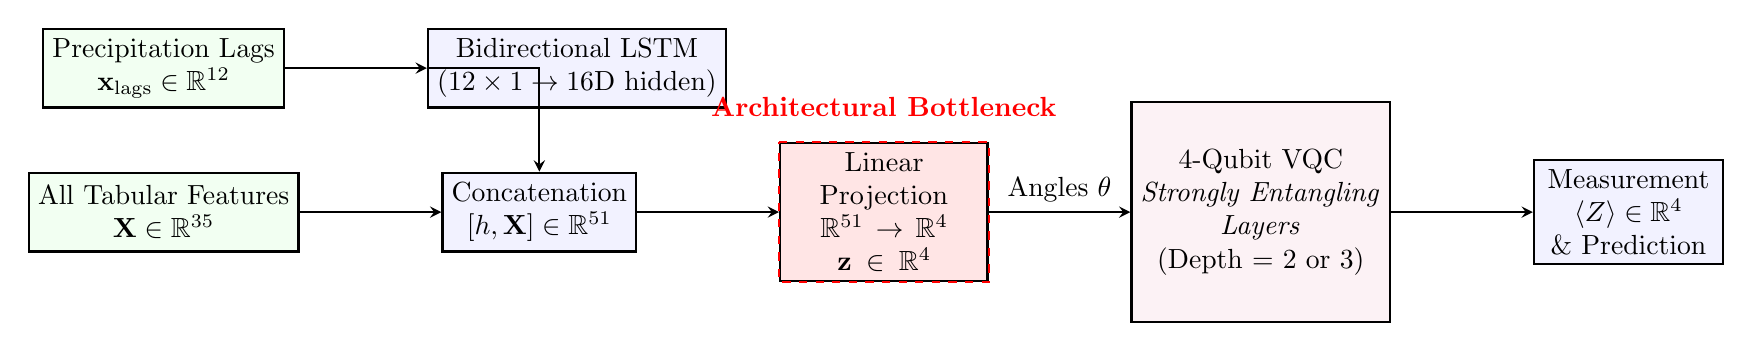
\begin{tikzpicture}[
        node distance=1.2cm and 1.8cm,
        box/.style={rectangle, draw=black, thick, minimum width=2.4cm, minimum height=1cm, align=center, fill=blue!5},
        quantum/.style={rectangle, draw=black, thick, minimum width=2.4cm, minimum height=2.8cm, align=center, fill=purple!5},
        arrow/.style={thick,->,>=stealth}
    ]
    \node (lags) [box, fill=green!5] {Precipitation Lags \\ $\mathbf{x}_{\text{lags}} \in \mathbb{R}^{12}$};
    \node (lstm) [box, right=of lags] {Bidirectional LSTM \\ ($12 \times 1 \to 16\text{D}$ hidden)};
    \node (features) [box, below=0.8cm of lags, fill=green!5] {All Tabular Features \\ $\mathbf{X} \in \mathbb{R}^{35}$};
    \node (concat) [box, right=of features] {Concatenation \\ $[h, \mathbf{X}] \in \mathbb{R}^{51}$};
    \node (bottleneck) [box, right=of concat, fill=red!10, text width=2.4cm] {Linear Projection \\ $\mathbb{R}^{51} \to \mathbb{R}^{4}$ \\ $\mathbf{z} \in \mathbb{R}^{4}$};
    \node (vqc) [quantum, right=of bottleneck] {4-Qubit VQC \\ \textit{Strongly Entangling} \\ \textit{Layers} \\ (Depth = 2 or 3)};
    \node (output) [box, right=of vqc] {Measurement \\ $\langle Z \rangle \in \mathbb{R}^4$ \\ \& Prediction};
    
    \draw [arrow] (lags) -- (lstm);
    \draw [arrow] (lstm) -| (concat);
    \draw [arrow] (features) -- (concat);
    \draw [arrow] (concat) -- (bottleneck);
    \draw [arrow] (bottleneck) -- node[above] {Angles $\theta$} (vqc);
    \draw [arrow] (vqc) -- (output);
    
    \draw[dashed, red, thick] (bottleneck.north west) -- (bottleneck.north east) -- (bottleneck.south east) -- (bottleneck.south west) -- cycle;
    \node[above=0.2cm of bottleneck, text=red, font=\bfseries] {Architectural Bottleneck};
    \end{tikzpicture}%
    }
    \caption{Hybrid Quantum-Classical Architecture. The bidirectional LSTM processes the univariate 12-month precipitation lag sequence ($\mathbf{x}_{\text{lags}} \in \mathbb{R}^{12}$), producing a 16-dimensional recurrent representation. This is concatenated with the full 35-dimensional tabular feature vector (which redundantly contains the 12 lags alongside physical covariates and station indicators) to form a 51-dimensional representation. A classical linear projection ($\mathbb{R}^{51} \to \mathbb{R}^4$) then compresses the features into 4 continuous rotation angles for encoding into the 4-qubit Variational Quantum Circuit.}
    \label{fig:architecture}
\end{figure}

\begin{figure}[htbp]
    \centering
    \resizebox{0.95\textwidth}{!}{%
    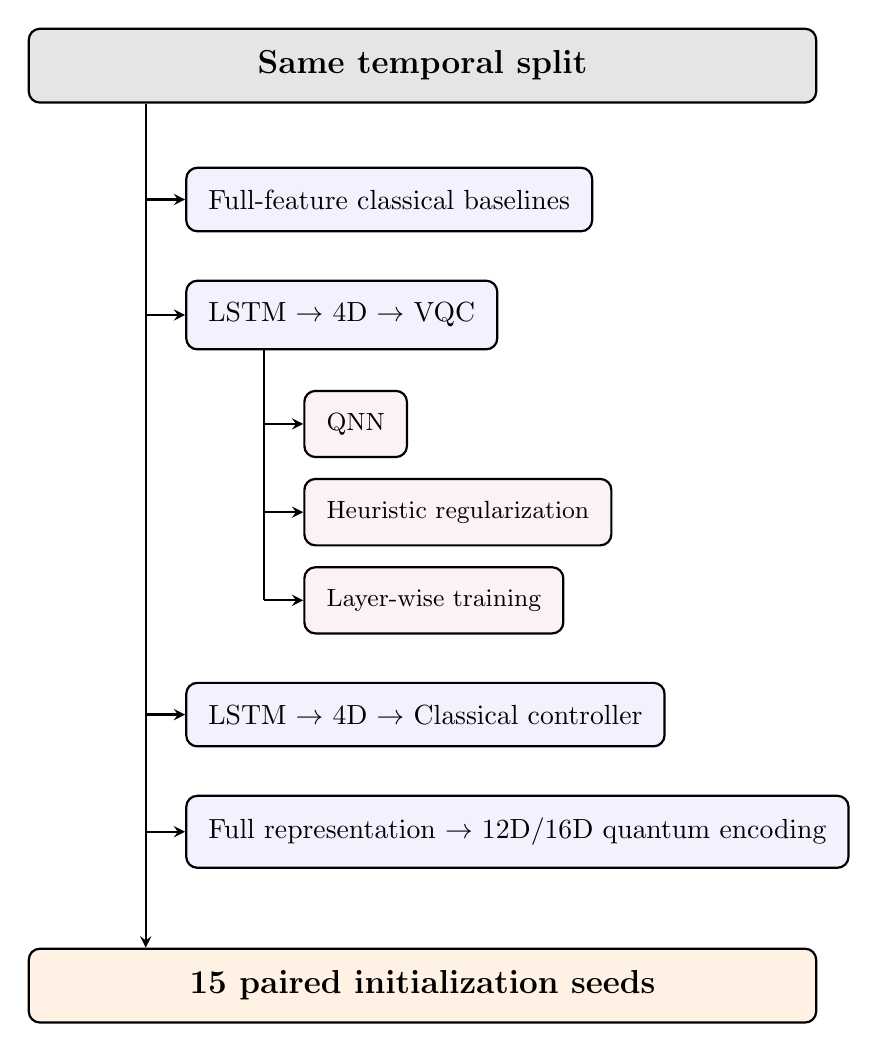
\begin{tikzpicture}[
        >=stealth,
        % Global node styles
        box/.style={rectangle, draw=black, thick, rounded corners, fill=white, inner sep=8pt, align=left, font=\normalsize},
        root/.style={box, fill=gray!20, font=\bfseries\large, align=center, minimum width=10cm},
        l1/.style={box, fill=blue!5},
        l2/.style={box, fill=purple!5, font=\small},
        seed/.style={box, fill=orange!10, font=\bfseries\large, align=center, minimum width=10cm}
    ]

    % ==========================================
    % 1. NODES DEFINITION
    % ==========================================
    
    % ROOT NODE
    \node[root] (split) {Same temporal split};

    % Define the X coordinate for the main vertical backbone
    \coordinate (L1_x) at ([xshift=1.5cm]split.south west);

    % LEVEL 1: Baselines
    \node[l1, anchor=north west] (class) at ([xshift=0.5cm, yshift=-0.8cm]L1_x) {Full-feature classical baselines};

    % LEVEL 1: VQC Base
    \node[l1, anchor=north west] (vqc) at ([yshift=-0.6cm]class.south west) {LSTM $\rightarrow$ 4D $\rightarrow$ VQC};

        % Define the X coordinate for the VQC sub-backbone
        \coordinate (VQC_branch) at ([xshift=1cm]vqc.south west);

        % LEVEL 2: VQC Branches
        \node[l2, anchor=north west] (qnn) at ([xshift=0.5cm, yshift=-0.5cm]VQC_branch |- vqc.south) {QNN};
        \node[l2, anchor=north west] (phys) at ([yshift=-0.25cm]qnn.south west) {Heuristic regularization};
        \node[l2, anchor=north west] (lbl) at ([yshift=-0.25cm]phys.south west) {Layer-wise training};

    % LEVEL 1: Classical Controller Control
    % We use (lbl.south -| class.west) to ensure it stays below the L2 nodes but aligns left with L1
    \node[l1, anchor=north west] (control) at ([yshift=-0.6cm]lbl.south -| class.west) {LSTM $\rightarrow$ 4D $\rightarrow$ Classical controller};

    % LEVEL 1: Bandwidth Extension
    \node[l1, anchor=north west] (enc) at ([yshift=-0.6cm]control.south west) {Full representation $\rightarrow$ 12D/16D quantum encoding};

    % BOTTOM NODE: Seeds
    % Centered relative to the root node
    \node[seed, anchor=north] (seeds) at ([yshift=-1cm]enc.south -| split.center) {15 paired initialization seeds};

    % ==========================================
    % 2. PATH DRAWING (ARROWS)
    % ==========================================

    % Main vertical backbone 
    \draw[thick] (L1_x) -- (L1_x |- enc.west);
    
    % The backbone continues down to hit the top of the 'seeds' box
    \draw[thick, ->] (L1_x |- enc.west) -- (L1_x |- seeds.north);

    % Horizontal branches to Level 1
    \draw[thick, ->] (L1_x |- class.west) -- (class.west);
    \draw[thick, ->] (L1_x |- vqc.west) -- (vqc.west);
    \draw[thick, ->] (L1_x |- control.west) -- (control.west);
    \draw[thick, ->] (L1_x |- enc.west) -- (enc.west);

    % VQC vertical sub-backbone
    \draw[thick] (VQC_branch) -- (VQC_branch |- lbl.west);
    
    % Horizontal branches to Level 2
    \draw[thick, ->] (VQC_branch |- qnn.west) -- (qnn.west);
    \draw[thick, ->] (VQC_branch |- phys.west) -- (phys.west);
    \draw[thick, ->] (VQC_branch |- lbl.west) -- (lbl.west);

    \end{tikzpicture}%
    }
    \caption{Schematic of the experimental design. All evaluated architectures originate from the identical temporal split and culminate in a rigorous 15-seed parameter initialization protocol to control for optimization variance. The hierarchy explicitly isolates the full-feature classical baselines from the hybrid quantum models, and pairs the latter with bottleneck-matched classical controls and encoding-bandwidth ablations.}
    \label{fig:experimental_design}
\end{figure}

To test whether domain-motivated soft constraints alter optimization trajectories, we evaluate two hybrid configurations incorporating heuristic thermodynamic regularization (\texttt{LSTM+PI-QNN} and \texttt{LbL-QNN}). As detailed in \Cref{app:heuristic_regularization}, this scheme supplements binary cross-entropy with two phenomenological soft penalties: a temperature-dependent gating term ($\mathcal{L}_{\text{CC}}$) penalizing high precipitation predictions under restricted saturation-capacity conditions, and a latent-coordinate balance term ($\mathcal{L}_{\text{hMSE}}$) acting on the 4-qubit expectation readout coordinates ($q_0, \dots, q_3$). These are empirical soft regularizers rather than first-principles thermodynamic conservation laws. As shown in \Cref{sec:stability}, 15-seed replication reveals that this heuristic regularization confers no statistically significant performance advantage over the unconstrained hybrid baseline (Friedman $p = 0.458$).

\subsection{Quantum and Classical Architectures}
\label{app:architectures}

We evaluate ten distinct model architectures alongside one threshold-matched operational configuration (yielding eleven evaluation configurations in \Cref{tab:single_run_results}), grouped into four paradigms:
\begin{enumerate}
    \item \textbf{Statistical and Climatological Reference Baselines:} We evaluate non-parametric reference benchmarks alongside $L_2$-regularized Logistic Regression: (i) \emph{Month $\times$ Station Climatology}, which assigns each test sample the empirical frequency of precipitation exceeding $P_{60}$ observed for that specific station and calendar month in the training partition (AUC = 0.680, Brier score = 0.222, Brier skill score relative to the sample base rate = $+0.082$); and (ii) \emph{Climatological Persistence}, evaluated as an unranked binary baseline thresholded at 0.5 ($\text{Acc} = 64.58\%$, $\text{F1} = 0.522$, binary $\text{AUC} = 0.619$), whereas physical lag-1 precipitation persistence achieves $\text{AUC} = 0.589$.

    \item \textbf{Classical Ensembles:} Random Forest (300 estimators), Gradient Boosting (200 estimators), and XGBoost (500 estimators, depth=4).
    \item \textbf{Deep Learning Baselines:} A standalone bidirectional LSTM (\texttt{PureLSTM}) with 2 layers and 16 hidden units per direction (yielding a concatenated 32-dimensional sequence representation), concatenated with the 35 input features (67 dimensions), followed by batch normalization (\texttt{BatchNorm1d(67)}) and a two-layer classification head (\texttt{Linear(67, 16)} + LayerNorm + \texttt{Linear(16, 1)}), totaling 10,103 parameters, optimized using AdamW. Alongside this model, we evaluate \texttt{Matched LSTM}, an operational configuration of \texttt{PureLSTM} with its classification threshold adjusted to match the false positive rate of the hybrid models ($\tau = 0.531$; \Cref{app:operational_analysis}). We emphasize that the standalone LSTM is not capacity-matched to the hybrids (10,103 vs.\ $\sim$2,600 parameters; 16 vs.\ 8 hidden units per direction; batch normalization; and direct access to raw features without a 4-dimensional projection bottleneck).
    \item \textbf{Hybrid Quantum-Classical Models:} Developed using PennyLane's \texttt{default.qubit} simulator. All models use a bidirectional LSTM (hidden dimension 8 per direction, 2,368 parameters) concatenated with the 35 input features to produce a 51-dimensional representation, which is compressed via a linear layer (\texttt{Linear(51, 4)}, 208 parameters) into a 4-dimensional projection bottleneck before being encoded into a 4-qubit Variational Quantum Circuit. The circuit uses a Strongly Entangling Layers ansatz with same-vector data re-uploading ($R_y$ and $R_z$ rotations per qubit repeated in each layer; \citealp{perez2020}) followed by parameterized $\mathrm{SU}(2)$ $\mathrm{Rot}$ gates and a circular CNOT entanglement topology ($L = 2$ layers with 24 quantum parameters for baseline models; $L = 3$ layers with 36 quantum parameters for the layer-wise \texttt{LbL-QNN} model; see \Cref{fig:vqc_circuit}). We distinguish this repeated encoding from the \emph{information-widening} re-uploading variant introduced later (\Cref{sec:relaxing_bottleneck}), which injects distinct feature subsets at each block.
    \begin{itemize}
        \item \texttt{LSTM+QNN}: Standard end-to-end unconstrained variational network (2 layers).
        \item \texttt{LSTM+PI-QNN}: End-to-end network optimized with the heuristic thermodynamic loss $\mathcal{L}_{\text{total}}$ (2 layers; \Cref{app:heuristic_regularization}).
        \item \texttt{LSTM+QTL}: Quantum Transfer Learning \citep{mari2020}, where the classical LSTM features are frozen and only a lightweight classical adapter feeding the quantum layer is optimized (2 layers).
        \item \texttt{LbL-QNN}\footnote{This architecture combines layer-by-layer training \citep{skolik2021} with the heuristic thermodynamic loss (\Cref{app:heuristic_regularization}). As shown in \Cref{app:depth_justification}, a depth-matched ablation specifically evaluating \texttt{LbL-QNN} against an end-to-end 3-layer architecture (\texttt{LSTM+PI-QNN-3L}) confirms its stability benefit is not attributable to circuit depth alone. However, this comparison is confounded by an expanded training budget (55 total epochs: 10 epochs per layer across 3 layers = 30 epochs, followed by 25 global fine-tuning epochs vs.\ 25 single-run epochs) and a staged learning rate schedule ($5\times 10^{-3}$ then $5\times 10^{-4}$ vs.\ fixed $5\times 10^{-3}$). The observed variance stabilization is therefore associated with the combined multi-stage schedule and expanded budget rather than demonstrably caused by the layer-wise inductive bias in isolation, particularly since a penalty-free layer-by-layer control and an epoch-matched (55-epoch) end-to-end control were not evaluated; the observed performance should be attributed to the combined layer-wise/heuristic configuration.}: applies the layer-by-layer training protocol to the \texttt{LSTM+PI-QNN} architecture, using a 3-layer circuit to support a non-degenerate three-stage freezing schedule.
        \item \texttt{QKSVM}: Quantum Kernel Support Vector Machine utilizing a Nystr\"{o}m approximation ($M=64$ landmarks) to handle the panel's size.
    \end{itemize}
\end{enumerate}

\begin{figure}[htbp]
    \centering
    \resizebox{\textwidth}{!}{%
    \begin{quantikz}[row sep=0.5cm, column sep=0.45cm]
        \lstick{$\ket{0}_{q_0}$} &
        \gategroup[wires=4, steps=2, style={dashed, rounded corners, fill=blue!5, inner sep=6pt}, background, label style={label position=above, anchor=south, yshift=0.2cm}]{\makebox[0pt]{Data Encoding}} \gate{R_y(x_0)} & \gate{R_z(x_0)} &
        \gategroup[wires=4, steps=5, style={dashed, rounded corners, fill=purple!5, inner sep=6pt}, background, label style={label position=above, anchor=south, yshift=0.2cm}]{\makebox[0pt]{Variational Ansatz}} \gate{\mathrm{Rot}(\vec\theta_0)} &
        \ctrl{1} & \qw & \qw & \targ{} & \meter{} \\
        \lstick{$\ket{0}_{q_1}$} & \gate{R_y(x_1)} & \gate{R_z(x_1)} & \gate{\mathrm{Rot}(\vec\theta_1)} & \targ{} & \ctrl{1} & \qw & \qw & \meter{} \\
        \lstick{$\ket{0}_{q_2}$} & \gate{R_y(x_2)} & \gate{R_z(x_2)} & \gate{\mathrm{Rot}(\vec\theta_2)} & \qw & \targ{} & \ctrl{1} & \qw & \meter{} \\
        \lstick{$\ket{0}_{q_3}$} & \gate{R_y(x_3)} & \gate{R_z(x_3)} & \gate{\mathrm{Rot}(\vec\theta_3)} & \qw & \qw & \targ{} & \ctrl{-3} & \meter{}
    \end{quantikz}%
    }
    \caption{Gate-level schematic of a single layer of the 4-qubit Variational Quantum Circuit
    (VQC). The 4-dimensional classical bottleneck vector $\mathbf{x}$ is injected into the quantum
    state via consecutive $R_y(x_i)$ and $R_z(x_i)$ rotations on each qubit (Data Encoding; \citealp{perez2020}). The trainable ansatz consists of general
    $\mathrm{SU}(2)$ rotations ($\mathrm{Rot}$ gates, each parameterized by a 3-component vector
    $\vec\theta_i = (\theta_{i,1}, \theta_{i,2}, \theta_{i,3})$) followed by a circular CNOT
    entanglement topology. To implement the Strongly Entangling Layers architecture, this entire
    encoding-ansatz block is repeated $L$ times (with $L=2$ for the baseline models, yielding 24 quantum parameters, and $L=3$ for
    the layer-wise \texttt{LbL-QNN} model, yielding 36 quantum parameters). Readout is performed via Pauli-$Z$ measurements on
    all qubits.}
    \label{fig:vqc_circuit}
\end{figure}

\subsection{Bottleneck-Controlled Classical Baseline}
\label{sec:bottleneck_control}\label{app:bottleneck}

A central confound in comparing hybrid quantum architectures against full-feature classical
ensembles is that the VQC-based models operate on a 4-dimensional projection produced by the LSTM
bottleneck, whereas classical ensembles ingest the full 35-dimensional engineered feature space,
including geographic fixed effects.

To isolate this confound, we evaluate three bottleneck-matched classical control configurations
(\texttt{LSTM+MLP-4D}) spanning a range of parameter counts. These architectures are identical to
\texttt{LSTM+QNN} in their upstream feature extractor, 4-dimensional projection bottleneck, and
downstream classification head, but replace the 4-qubit VQC with a classical controller (linear,
LeakyReLU, or GELU MLP). All configurations were replicated across the same 15 seed-paired
initializations used for \texttt{LSTM+QNN} (\Cref{tab:bottleneck_control}). An initial width-2 ReLU-based control collapsed to
chance-level output (AUC$=0.500$) in 9 of 15 seeds due to dead-unit failure; we resolved this with
the linear and LeakyReLU configurations reported below, confirming the failure was
activation-specific, not capacity-related (full diagnostic in \Cref{app:relu_collapse}).

We emphasize that parameter count is a coarse and imperfect proxy for functional capacity: a
linear model and a nonlinear, GELU-activated MLP with comparable parameter counts are not
necessarily comparable in expressive power, since capacity depends jointly on activation
nonlinearity and architecture, not on parameter count alone. We therefore describe these three
controls as spanning a range of parameter counts and architectural nonlinearities, rather than as
strictly bottleneck-controlled to the quantum circuit in a formal sense. The qualitative conclusion
below is nonetheless robust to this caveat, as the absence of a statistically significant difference from the quantum
circuit holds independently for both the least expressive (linear) and most expressive (GELU)
control considered.

\begin{table}[htbp]
\centering
\caption{Bottleneck-controlled comparison: classical controls versus the quantum circuit under an
identical 4-dimensional information bottleneck, versus the full-feature Random Forest reference,
sorted descending by mean AUC. All values are 15-seed distributions with seed-paired initialization.}
\label{tab:bottleneck_control}
{\small
\setlength{\tabcolsep}{4.5pt}
\begin{tabular}{lcccc}
\toprule
\textbf{Architecture} & \textbf{Controller params} & \textbf{Mean AUC} & \textbf{Std. Dev.} & \textbf{Max} \\
\midrule
Random Forest (matched, 2,273 rows)\textsuperscript{*} & Ensemble & 0.6802 & 0.0035 & 0.687 \\
Random Forest (train+val, 2,787 rows)\textsuperscript{*} & Ensemble & 0.6851 & 0.0026 & 0.690 \\
LSTM+QNN (quantum, 4-dim. bottleneck) & 24 & 0.6589 & 0.0153 & 0.681 \\
GELU MLP (classical control, 4-dim. input) & 180 & 0.6563 & 0.0071 & 0.6725 \\
Linear (classical control, 4-dim. input) & 20 & 0.6545 & 0.0069 & 0.6680 \\
LeakyReLU MLP (classical control, 4-dim. input) & 28 & 0.6516 & 0.0083 & 0.6636 \\
\bottomrule
\end{tabular}%
}
\vspace{4pt}

{\footnotesize\textsuperscript{*}Tree ensemble capacity is determined by the number of leaves/nodes rather than differentiable parameters; the 300-tree Random Forest with \texttt{max\_depth=8} possesses a functional capacity vastly exceeding the 24 parameters of the quantum circuit. The 2,273-row model provides the strictly matched training comparison to the neural and hybrid models. Parameter counts reported under Controller params reflect only the 4-dimensional controller/neck replacing the quantum circuit; for total model parameter accounting (including the shared 2,589 classical backbone), see \Cref{tab:parameter_accounting}.}
\end{table}

A 4-qubit circuit with 24 variational parameters operates on a state space of dimension $2^4 = 16$; its statevector evolution is represented by a $16 \times 16$ unitary matrix, which is classically simulable in sub-millisecond time. Functionally, parameterized quantum circuits with angle encoding compute truncated Fourier series of the input coordinates \citep{schuld2022}, so that classical models with periodic or trigonometric activations ($\cos, \sin$) and matched parameter capacity ($\sim 24$ weights) serve as direct functional analogues. 

To evaluate whether the lack of a statistically significant difference between classical controls and the quantum circuit reflects statistical equivalence, we conducted Two One-Sided Tests (TOST) against \texttt{LSTM+QNN} across the 15 seeds. Under a primary equivalence margin of $\Delta = \pm 0.010$ AUC, \texttt{GELU MLP-4D} achieves formal equivalence ($\text{Diff} = -0.0025$, paired 90\% CI $[-0.0092, +0.0041]$, $p_{\text{TOST}} = 0.0350$). The smaller \texttt{Linear-4D} ($\text{Diff} = -0.0044$, 90\% CI $[-0.0121, +0.0032]$, $p_{\text{TOST}} = 0.1113$) and \texttt{LeakyReLU-4D} ($\text{Diff} = -0.0073$, 90\% CI $[-0.0151, +0.0005]$, $p_{\text{TOST}} = 0.2772$) do not reject the $\pm 0.010$ margin. However, under a sensitivity margin of $\Delta = \pm 0.015$ AUC, \texttt{Linear-4D} also achieves formal equivalence ($p_{\text{TOST}} = 0.0148$), and under $\Delta = \pm 0.020$ AUC all three classical controllers are statistically equivalent to the quantum circuit ($p_{\text{TOST}} \le 0.0064$). Wilcoxon signed-rank tests similarly show no significant differentiation ($p \in [0.17, 0.64]$), which is consistent with the absence of a measurable circuit effect at the fixed 4-dimensional interface. As in \Cref{sec:applying}, these seed-level tests omit test-set sampling error and the margins used are below the MDE of \Cref{sec:budget}; all three paired 90\% intervals lie within $\pm 0.016$ AUC.

We additionally evaluated classical controls under an unsupervised 4-dimensional compression of the entire 35-dimensional input space, providing an information-matched benchmark for \texttt{QKSVM} (\Cref{sec:architectures}). Fitting Principal Component Analysis strictly on the training partition ($\text{PCA}(4)$, capturing 65.70\% of total variance across the 35 features) and evaluating on the test partition, a classical Support Vector Machine with an RBF kernel achieves an AUC of 0.6686 and a Brier score of 0.2219 (with $\text{Acc} = 62.31\%$, $\text{F1} = 0.5158$, and $\text{Rc-ACP} = 0.8500$). This classical 4-dimensional benchmark outperforms the 4-qubit Quantum Kernel SVM (AUC = 0.6390, Brier score = 0.2283; \Cref{tab:single_run_results}) by 0.030 AUC, a gap below the MDE of \Cref{sec:budget}, whereas tree ensembles on PCA-4 achieve lower discriminative performance (Random Forest: $0.6312 \pm 0.0030$; Gradient Boosting: $0.6230 \pm 0.0005$). This indicates that the modest score of \texttt{QKSVM} is not explained by low-dimensional compression alone; whether it reflects the inductive bias of the evaluated quantum feature map cannot be resolved at this noise level.

Random Forest is not a bottleneck-matched comparator for the VQC; it operates on the uncompressed 35-dimensional space with 300 trees, establishing an empirical tabular reference (Mean AUC $= 0.6802 \pm 0.0035$ on matched 2,273 rows; $0.6851 \pm 0.0026$ on 2,787 rows). The 4D controls hold the input interface constant, isolating circuit-specific effects from representation compression: at this fixed interface, classical controllers demonstrate equivalence to the quantum circuit within $\pm 0.015$ AUC. While restricting models to a 4D interface degrades performance relative to Random Forest, the information bottleneck alone cannot explain the classical-over-quantum gap, because full-feature tree ensembles such as XGBoost ($0.6575 \pm 0.0051$) achieve discriminative performance comparable to baseline \texttt{LSTM+QNN} ($0.6589 \pm 0.0153$). The residual gap to Random Forest may reflect model-family capabilities on tabular data rather than an encoding bottleneck, and is itself below the MDE.

As exploratory evidence on whether the 4-dimensional compression itself constrains the recurrent backbone, we also evaluated a bottleneck-free classical LSTM with the same hidden dimension 8 (\texttt{bottleneck\_free\_lstm}, arithmetically $\sim$2,522 parameters: 2,368 LSTM + 102 BatchNorm + 52 linear head, though parameter counts were not stored in the checkpoint). Unlike the hybrid, which projects the 51-dimensional representation (16D LSTM hidden + 35D raw features) down to 4 dimensions before classification, this model attaches a direct linear classification head to the 51-dimensional vector. Across 15 seeds, it achieves an AUC of $0.6435 \pm 0.0065$. Because the classifier head differs and no paired seed-by-seed test was logged, this exploratory result does not support a claim that removing the bottleneck formally confirms compression as a performance limit. Descriptively, the bottleneck-free model falls below both the 4D linear control ($0.6545 \pm 0.0069$) and the 4D MLP controls ($0.6563 \pm 0.0071$, $0.6516 \pm 0.0083$), as well as the larger Standalone LSTM ($0.6657 \pm 0.0091$). That the 4D linear control scores 0.011 above the unprojected 51D head (a gap below the MDE) at most suggests that low-dimensional linear projection can act as a regularizer for this small recurrent backbone, rather than compression acting solely as an upper bound on performance. We explicitly separate the claim of projection regularization from the claim that quantum circuits provide an inductive advantage at that interface.

The training protocol reveals an important asymmetry between model families: tree ensembles (Random Forest, Gradient Boosting, and XGBoost) were originally fit on the 2,787 rows of the combined training and validation partitions ($X_{\text{sk}} = X_{\text{all}}[:s_2]$), whereas neural and hybrid quantum models were fit on the 2,273 training rows with validation rows reserved for early stopping (\Cref{sec:validation_protocol}). Evaluating Random Forest strictly on the 2,273 training rows with canonical hyperparameters yields a 15-seed mean AUC of $0.6802 \pm 0.0035$ (range $[0.6732, 0.6867]$), compared to $0.6851 \pm 0.0026$ on 2,787 rows. An automated Optuna search (50 trials) on the 2,273 training rows yielded $0.6798 \pm 0.0045$. We report both: the primary Random Forest of the main text is the train-only pipeline fitted on 2,787 rows, and the 2,273-row model is a sensitivity analysis whose 0.005 lower AUC is within the noise of the benchmark.


% ============================================================
\section{Additional Results}
\label{app:additional_results}
% ============================================================

\subsection{Single-Run Performance}
\label{sec:single_run}

We evaluate model performance on the canonical spatiotemporal test partition ($N=528$ station-months, 2008--2026) using the canonical dataset \texttt{01\_data.pt} ($P_{60}=28.1$, $P_{90}=86.32$\,mm). As established by our 15-seed replication rerun on the canonical dataset (\Cref{app:leakage_correction}), adopting a strict train-only standardization protocol yields downstream performance deltas of small magnitude ($\le 0.004$ AUC) and mixed sign across model families, reflecting optimization seed variability rather than systematic leakage inflation.

\Cref{tab:single_run_results} summarizes the single-run test performance across all evaluated models at a fixed initialization seed (\texttt{seed=42}). Global accuracy is misleading due to class imbalance; we therefore focus on F1-score, ROC-AUC, and Precision-Recall AUC (PR-AUC; \citealp{davis2006,saito2015}). The tree-based \textbf{Random Forest} establishes the classical reference across ROC-AUC and F1 (AUC = 0.688, F1 = 0.603), while the non-parametric \textbf{Month $\times$ Station Climatology} establishes an empirical baseline that matches or exceeds all quantum models (AUC = 0.680, PR-AUC = 0.603). The hybrid quantum-classical architectures cluster tightly below (AUC: 0.639--0.672; F1: 0.580--0.604).

\begin{table}[htbp]
\centering
\caption{Comparative performance on the spatiotemporal test set (Single-Run), including Precision-Recall AUC (PR-AUC) alongside ROC-AUC. Single representative run evaluated at default threshold 0.5 ($n=20$ ACP-flagged test months exceeding $P_{60}$ out of 25 flagged total; $n=49$ $P_{90}$-exceeding test months). Month $\times$ Station Climatology establishes the non-parametric empirical baseline.}
\label{tab:single_run_results}
\setlength{\tabcolsep}{4.5pt}
\begin{tabular}{l c c c c c c c}
\toprule
\textbf{Model} & \textbf{Acc (\%)} & \textbf{F1} & \textbf{ROC-AUC} & \textbf{PR-AUC} & \textbf{Rc-$P_{90}$} & \textbf{Rc-ACP} & \textbf{FPR} \\
\midrule
\multicolumn{8}{l}{\textit{Climatological Reference}}\\
Month $\times$ Station Climatology & 61.2 & 0.547 & 0.680 & \textbf{0.603} & 0.653 & 0.600 & 0.360 \\
\midrule
\multicolumn{8}{l}{\textit{Statistical \& Ensemble}}\\
Logistic Regression & 62.3 & 0.472 & 0.655 & 0.546 & 0.571 & 0.650 & 0.228 \\
Random Forest & 63.8 & 0.603 & \textbf{0.688} & 0.591 & 0.755 & 0.900 & 0.383 \\
Gradient Boosting & 61.6 & 0.522 & 0.671 & 0.577 & 0.592 & 0.700 & 0.312 \\
XGBoost & 59.1 & 0.548 & 0.650 & 0.545 & 0.694 & 0.850 & 0.418 \\
\midrule
\multicolumn{8}{l}{\textit{Deep Learning}}\\
Standalone LSTM & 54.5 & 0.585 & 0.653 & 0.587\textsuperscript{*} & 0.816 & 0.950 & 0.617 \\
Matched LSTM$^{\dagger}$ & 57.2 & 0.565 & 0.653 & 0.587\textsuperscript{*} & 0.776 & 0.950 & 0.502 \\
\midrule
\multicolumn{8}{l}{\textit{Quantum-Classical Hybrid}}\\
LSTM+QNN & 58.0 & 0.599 & 0.639 & 0.504 & 0.796 & 0.950 & 0.550 \\
LSTM+PI-QNN & 58.9 & 0.583 & 0.662 & 0.558 & 0.755 & 0.950 & 0.489 \\
LSTM+QTL & 58.7 & 0.604 & 0.651 & 0.518 & 0.837 & 0.850 & 0.537 \\
\textbf{LbL-QNN} & 59.1 & 0.589 & 0.672 & 0.581 & 0.796 & 0.900 & 0.495 \\
QKSVM & 59.8 & 0.475 & 0.639 & 0.510 & 0.612 & 0.600 & 0.293 \\
\bottomrule
\end{tabular}
\vspace{4pt}

{\footnotesize
\textsuperscript{*}PR-AUC is threshold-independent and therefore identical to the unmatched Standalone LSTM row; only the operational point (FPR, recall) changes under matching.\par
\textsuperscript{$\dagger$}Threshold-recalibrated variant of Standalone LSTM, evaluated at an operating point matched in false-positive rate to \texttt{LbL-QNN} ($\tau = 0.531$); defined and motivated in \Cref{app:operational_analysis}.\par
Rc-ACP is evaluated strictly over the $n=20$ positive test months ($y=1$) matching the Autumn Convective Proxy in the canonical pipeline (out of 25 flagged months total), distinct from the 32 flagged months (25 positive) identified under train-only anomaly standardization (\Cref{app:leakage_correction}); if all 25 flagged months are counted regardless of precipitation (the alarm rate), the respective values are: Climatology 0.640, Logistic Regression 0.600, Random Forest 0.880, Gradient Boosting 0.680, XGBoost 0.840, Standalone LSTM 0.960, Matched LSTM 0.960, LSTM+QNN 0.920, LSTM+PI-QNN 0.960, LSTM+QTL 0.840, LbL-QNN 0.920, QKSVM 0.520.
}
\end{table}

In this single realization, the layer-wise hybrid \texttt{LbL-QNN} achieves the highest quantum AUC (0.672), tracking Random Forest (\Cref{tab:single_run_results}) with no statistically significant difference under an uncorrected DeLong test \citep{delong1988} ($p = 0.2124$; formal equivalence not tested). It nominally outperforms unconstrained \texttt{LSTM+QNN} ($p = 0.0070$) and \texttt{Standalone LSTM} ($p = 0.0263$), though the latter comparison is heavily confounded by the capacity mismatch (10,103 vs.\ $\sim$2,600 parameters; \Cref{sec:architectures}).

Crucially, this apparent single-run superiority dissolves under closer examination. First, comparing Random Forest to Month $\times$ Station Climatology yields no statistically significant advantage under a paired DeLong test ($\Delta \text{AUC} = +0.0079$, $\text{SE} = 0.0177$, $z = 0.449$, $p = 0.6534$). Accounting for temporal dependence via a year-block bootstrap ($B=2{,}000$ resamples of the 19 test calendar years 2008--2026; \citealp{kunsch1989}), the difference remains non-significant ($\Delta \text{AUC} = +0.0068$, $95\%$ block CI: $[-0.0171, +0.0284]$, $p = 0.5420$). Thus, neither Random Forest nor any evaluated quantum architecture demonstrates statistically verifiable predictive skill beyond empirical seasonal-geographic climatology when temporal autocorrelation is respected.

Second, disaggregating test performance across individual monitoring stations reveals that the pooled ROC-AUC ($N=528$) aggregates disparate regional regimes. In Alicante ($N=221$, $29.4\%$ positive rate), Random Forest achieves an AUC of 0.698 and \texttt{LbL-QNN} achieves 0.683, compared to 0.681 for Climatology. In Barcelona ($N=221$, $50.2\%$ positive rate), Climatology achieves an AUC of 0.663, outperforming both Random Forest (0.634) and all quantum models (\texttt{LbL-QNN}: 0.643; \texttt{LSTM+QNN}: 0.538). In Valencia ($N=50$, $56.0\%$ positive rate), Climatology (0.692) likewise exceeds Random Forest (0.690), \texttt{LbL-QNN} (0.649), and \texttt{LSTM+QNN} (0.607), while in San Javier ($N=36$, $36.1\%$ positive rate), all models cluster between 0.535 and 0.575. This indicates that a substantial fraction of pooled discriminative performance arises from separating high-base-rate from low-base-rate stations rather than dynamically resolving extreme months within a station regime.

Third, because the extreme tail contains limited test observations ($n=20$ ACP months exceeding $P_{60}$, $n=49$ $P_{90}$ months), point estimates of extreme recall carry wide 95\% Wilson confidence intervals that broadly overlap across all architectures (e.g., Random Forest $0.900$ [0.699, 0.972] vs.\ \texttt{LSTM+QNN} $0.950$ [0.764, 0.991]; documented in \Cref{app:operational_analysis}). Fourth, the apparent operational difference between \texttt{Standalone LSTM} (Rc-ACP = 0.950, FPR = 0.617) and \texttt{LbL-QNN} (Rc-ACP = 0.900, FPR = 0.495) is entirely an artifact of default threshold selection: recalibrating the classical LSTM to operate at an identical FPR of $\approx$50.2\% (\texttt{Matched LSTM}, $\tau = 0.531$) preserves its recall at 0.950 (19/20) with no statistically significant difference under paired bootstrap resampling ($n=2{,}000$; full analysis in \Cref{app:operational_analysis}). Finally, as demonstrated in \Cref{sec:stability}, multi-seed replication reveals that these single-run margins reflect initialization variance rather than robust architectural advantages.

\subsection{Probabilistic Verification, Calibration, and Spatiotemporal Block Resampling}
\label{sec:calibration_and_block_bootstrap}

Because extreme-precipitation forecasting is intrinsically probabilistic, threshold-dependent binary metrics must be supplemented by proper scoring rules and calibration diagnostics. Across the test partition ($N_{\text{test}}=528$), the non-parametric Month $\times$ Station Climatology establishes a competitive reference Brier score of $0.2224$ (Brier Skill Score $\text{BSS}_{\text{uncond}} = +0.0816$ relative to the unconditional training base rate $0.4017$, $\text{BS}_{\text{uncond}} = 0.2422$). Among trained models, tree ensembles achieve the lowest probability error (Random Forest: $\text{BS} = 0.2230$, $\text{BSS}_{\text{uncond}} = +0.0791$; Gradient Boosting: $\text{BS} = 0.2236$, $\text{BSS}_{\text{uncond}} = +0.0767$), closely matching empirical climatology. Logistic Regression ($\text{BS} = 0.2258$, Expected Calibration Error $\text{ECE} = 0.0418$) and \texttt{QKSVM} ($\text{BS} = 0.2283$, $\text{ECE} = 0.0511$) achieve superior probability calibration. In contrast, all hybrid quantum architectures and the standalone LSTM exhibit pronounced probability overconfidence ($\text{ECE} \in [0.112, 0.149]$; Brier scores between $0.2352$ for \texttt{LbL-QNN} and $0.2536$ for \texttt{LSTM+QNN}), resulting in negative skill scores relative to climatology ($\text{BSS}_{\text{clim}} \in [-0.058, -0.140]$).

Furthermore, because standard DeLong tests assume sample independence that may be compromised by temporal autocorrelation, we conducted a year-block bootstrap analysis ($B = 2{,}000$ resamples of the 19 test calendar years 2008--2026; \citealp{kunsch1989}). Resampling entire calendar years across all monitoring stations confirms that Random Forest significantly outperforms \texttt{LbL-QNN} ($\Delta \text{AUC} = +0.0151$, $95\%$ block CI: $[+0.0007, +0.0281]$, $p = 0.0400$) and Standalone LSTM ($\Delta \text{AUC} = +0.0350$, $95\%$ block CI: $[+0.0183, +0.0501]$, $p = 0.0010$). These are single-seed comparisons: the seed-to-seed spread of the same models (\Cref{sec:budget}) is of the order of the gaps reported. Meanwhile, Gradient Boosting shows no statistically significant difference from \texttt{LbL-QNN} under block resampling ($\Delta \text{AUC} = -0.0010$, $95\%$ block CI: $[-0.0335, +0.0315]$, $p = 0.9280$).


\subsection{Feature Importance and Station Indicators}

\label{sec:feature_importance}

To understand how classical ensembles exploit the feature space, we analyze feature importances across model families. For Random Forest, evaluating Gini feature importance (Mean Decrease in Impurity, MDI) reveals that physically derived thermodynamic features account for $53.8\%$ of total model importance (led by seasonal thermal contrast \texttt{choque\_clausius} at $6.4\%$, cumulative evapotranspiration \texttt{et0\_sum} at $5.3\%$, and temperature anomaly \texttt{t\_anomaly} at $3.7\%$). Antecedent precipitation lags contribute $37.1\%$, cyclic month encodings account for $5.3\%$, and geographic station indicator dummies contribute only $3.8\%$. In contrast, XGBoost gain assigns greater weight to station-specific geographic indicators and cyclic month encodings, followed by thermodynamic proxies.

At face value, the high ranking of geographic indicators in boosted trees might suggest classical ensembles owe their advantage specifically to geographic fixed effects unavailable to the dimension-constrained quantum bottleneck. We test this directly via a station-identity ablation and the capacity-spanning classical control (\Cref{sec:bottleneck_control}), and find it does \emph{not} hold: removing the station indicators does not degrade classical performance (full ablation in \Cref{app:spatial_ablations}), and a classical network restricted to the same 4-dimensional bottleneck performs statistically indistinguishably from the quantum circuit. A plausible reading is that classical ensembles use the full \emph{high-dimensional} feature space---thermodynamic, moisture-lag and seasonal signals---rather than geographic information specifically. This describes what the tree ensembles use; it does not establish that compression causes the gap to the hybrids (\Cref{sec:applying}).

\subsection{The 15-Seed Replication of the Quantum Tier}
\label{sec:stability}\label{app:multiseed}

To test the stability of the single-run findings, we replicated the training pipeline across 15
independent random-parameter initialization seeds for all gradient-optimized architectures,
using a seed-pairing protocol. For the PyTorch-based quantum and deep-learning
architectures, seed $i$ fixes an identical data-shuffling order and initialization-stream
position via a common \texttt{torch.manual\_seed} call, mechanically justifying paired
comparisons. For cross-paradigm comparisons against the scikit-learn-based classical ensembles
(\Cref{sec:classical_multiseed}), seed $i$ instead denotes a consistent nominal block index
rather than a mechanically shared random stream. \Cref{tab:quantum_multiseed,tab:operational_multiseed} and \Cref{fig:auc_violin} present the resulting distributions for the quantum tier.

An omnibus Friedman test reveals no statistically significant difference in discriminative power
among the four quantum architectures ($\chi^2(3) = 2.600$, $p = 0.458$). The effect size is
small (Kendall's $W = 0.058$; \citealp{demsar2006}). As an informal plausibility check on
whether this null result could reflect insufficient statistical power rather than a genuine
absence of differentiation, we note that the encoding-bandwidth experiment reported in
\Cref{sec:relaxing_bottleneck}, using a directly comparable design ($k=6$ architectures,
$n=15$ paired seeds, identical Friedman procedure), reached nominal significance at
$W = 0.174$---approximately threefold higher than the effect size observed here. We report this
comparison descriptively, as a heuristic sanity check on the plausibility of a genuine null,
rather than as a formal post-hoc power calculation; we did not conduct a Monte Carlo or
asymptotic power analysis for the Friedman test under this specific design, and flag this as a
natural methodological extension for future replications of this benchmark. The single-run AUC
of 0.672 for \texttt{LbL-QNN} is consistent with a favorable draw from the upper tail of its
initialization distribution. Pairwise Wilcoxon tests indicate that \texttt{LbL-QNN} is not
statistically superior to any unconstrained counterpart ($p \ge 0.547$ in all cases); notably,
unconstrained \texttt{LSTM+QNN} achieves the best mean rank of the four (2.200), with
\texttt{LbL-QNN} second (2.400).

To determine whether the absence of a statistically significant difference corresponds to
statistical equivalence, we conducted paired Two One-Sided Tests (TOST;
\citealp{schuirmann1987,lakens2017}) on seed-level AUC differences. For each model pair, let
\(d_i = \mathrm{AUC}_{A,i} - \mathrm{AUC}_{B,i}\) denote the paired difference across the
\(n=15\) matched initialization seeds. We tested \(H_{01}:\mu_d\le-\Delta\) and
\(H_{02}:\mu_d\ge+\Delta\) using one-sided paired \(t\)-tests at \(\alpha=0.05\), with
\(\Delta=\pm0.010\) AUC as the primary margin. Equivalence was concluded when both null
hypotheses were rejected, equivalently when the paired \(90\%\) confidence interval for the
mean difference \(\bar d\) lay entirely within \((-\Delta,+\Delta)\). The primary margin was
defined before conducting the equivalence analysis but was not preregistered;
\(\Delta=\pm0.015\) and \(\pm0.020\) are reported as sensitivity analyses. We also report a
nonparametric Wilcoxon signed-rank TOST and, descriptively, the proportion of the
paired-difference \(t\) sampling distribution contained within the ROPE; this is a frequentist
coverage diagnostic, not a Bayesian posterior probability. These analyses quantify equivalence
in mean seed-level AUC under the fixed test partition; they do not establish equivalence of
generalization to new periods or stations. For \texttt{LSTM+QNN} versus \texttt{PI-QNN-LbL},
the mean difference is \(-0.0016\) (with standard error \(\text{SE}_\Delta = 0.0045\), standard deviation of the paired difference \(\text{SD}_\Delta = 0.0173\), and paired seed correlation \(r \approx 0.05\)), with a paired \(90\%\) CI of
\([-0.0095,+0.0062]\) contained within the \(\pm0.010\) bounds
(\(p_{\mathrm{TOST}}=0.0407\); Wilcoxon TOST \(p=0.0416\); \(t\)-based ROPE coverage
\(94.9\%\)). Under sensitivity margins \(\Delta = \pm 0.015\) and \(\pm 0.020\), equivalence holds at the wider margins (\(p_{\text{TOST}} \le 0.0028\)). These tests concern seed-level optimization only: test-set sampling uncertainty is far larger (standard error of one AUC 0.023--0.027; \Cref{sec:budget}) and the margins used are below the MDE.

To quantify how single-run benchmarks generate illusory advantages, we analyzed the complete pairwise cross-seed comparison matrix ($15 \times 15 = 225$ pairs) between \texttt{LbL-QNN} and \texttt{LSTM+QNN}. Across all 225 realizations, \texttt{LbL-QNN} yields a higher test AUC than \texttt{LSTM+QNN} in 52.0\% of cases (117/225), whereas \texttt{LSTM+QNN} is higher in 48.0\% of cases (108/225)---a virtually symmetric distribution. Crucially, if an experimenter evaluated an arbitrary single seed pair using an uncorrected DeLong test ($\alpha = 0.05$), they would falsely claim statistically significant superiority of \texttt{LbL-QNN} over \texttt{LSTM+QNN} in 6.7\% of draws (15/225), and superiority of \texttt{LSTM+QNN} over \texttt{LbL-QNN} in 1.3\% of draws (3/225). In total, 8.0\% of arbitrary single-run comparisons between these two equivalent models generate false claims of algorithmic superiority.

The clearest secondary pattern emerging from the quantum tier is lower across-seed variability
for the combined layer-wise/heuristic configuration. A depth-matched control for
\texttt{LbL-QNN} (\texttt{LSTM+PI-QNN-3L}) indicates that this variance reduction is not
explained by circuit depth alone (Levene's test at matched 3-layer depth,
$F_{\text{Levene}} = 7.47$, $p=0.011$; full analysis in
\Cref{app:depth_justification}). Because a penalty-free layer-wise control was not evaluated,
the separate contributions of the layer-by-layer protocol, the heuristic penalty, and the
expanded training budget remain not fully identified by the present design. The multi-seed
replication provides no evidence that heuristic thermodynamic regularization lowers the
false-alarm rate: the mean FPR of \texttt{LbL-QNN} ($0.541 \pm 0.079$) shows no statistically
significant difference from the unconstrained \texttt{LSTM+QNN} ($0.531 \pm 0.083$; Wilcoxon
$p = 0.847$; equivalence not formally tested).

\begin{table}[htbp]
\centering
\caption{Global AUC distribution across 15 independent training-seed replications (quantum models
only), sorted descending by mean AUC. Standard deviation is the sample standard deviation ($n-1$ denominator).}
\label{tab:quantum_multiseed}
\begin{tabular}{lcccc}
\toprule
\textbf{Architecture} & \textbf{Mean AUC} & \textbf{Std. Dev.} & \textbf{Minimum} & \textbf{Maximum} \\
\midrule
LbL-QNN & 0.6605 & 0.0089 & 0.645 & 0.681 \\
LSTM+QNN & 0.6589 & 0.0153 & 0.628 & 0.681 \\
LSTM+PI-QNN & 0.6555 & 0.0172 & 0.605 & 0.673 \\
LSTM+QTL & 0.6519 & 0.0128 & 0.632 & 0.679 \\
\bottomrule
\end{tabular}
\end{table}

\begin{figure}[htbp]
    \centering
    \safefig{figura_auc_violin.pdf}{0.75\textwidth}
    \caption{Violin plots of AUC distributions across 15 seeds for the four quantum architectures.
    Mean differences are statistically non-significant and trivial in effect size (Friedman
    $\chi^2=2.600$, $p=0.458$; Kendall's $W=0.058$).}
    \label{fig:auc_violin}
\end{figure}

\begin{table}[htbp]
\centering
\caption{Operational metric distributions (mean $\pm$ across-seed sample standard deviation, ddof=1) across 15 training seeds at a default decision threshold of 0.5, for all gradient-optimized and ensemble architectures ($n=20$ ACP months exceeding $P_{60}$, $n=49$ $P_{90}$ months).}
\label{tab:operational_multiseed}
\begin{tabular}{lccc}
\toprule
\textbf{Architecture} & \textbf{FPR} & \textbf{Rc-ACP} & \textbf{Rc-$P_{90}$} \\
\midrule
\textit{Classical Ensembles}\\
Random Forest & $0.383 \pm 0.011$ & $0.867 \pm 0.041$ & $0.746 \pm 0.022$ \\
Gradient Boosting & $0.310 \pm 0.006$ & $0.700 \pm 0.000$ & $0.595 \pm 0.007$ \\
XGBoost & $0.408 \pm 0.013$ & $0.890 \pm 0.047$ & $0.706 \pm 0.024$ \\
\midrule
\textit{Deep Learning}\\
Standalone LSTM & $0.513 \pm 0.066$ & $0.910 \pm 0.081$ & $0.782 \pm 0.031$ \\
\midrule
\textit{Quantum-Classical Hybrid}\\
LSTM+QNN & $0.531 \pm 0.083$ & $0.877 \pm 0.068$ & $0.785 \pm 0.047$ \\
LSTM+PI-QNN & $0.531 \pm 0.048$ & $0.897 \pm 0.079$ & $0.796 \pm 0.052$ \\
LSTM+QTL & $0.489 \pm 0.075$ & $0.860 \pm 0.069$ & $0.762 \pm 0.050$ \\
LbL-QNN & $0.541 \pm 0.079$ & $0.867 \pm 0.070$ & $0.784 \pm 0.045$ \\
\bottomrule
\end{tabular}
\vspace{4pt}

{\footnotesize Rc-ACP is evaluated strictly on the $n=20$ positive test months ($y=1$) matching the Autumn Convective Proxy in the canonical pipeline (25 flagged total), distinct from the 32 flagged months (25 positive) under train-only standardization (\Cref{app:leakage_correction}).}
\end{table}

\textit{Note on operational variance:} Across-seed variance in FPR is substantially higher in
gradient-optimized models (LSTMs and quantum hybrids) than in stochastic tree ensembles. A
detailed variance decomposition and Levene's test confirming this asymmetry ($F_{\text{Levene}} = 28.47$, $p < 0.0001$) is
provided in \Cref{app:variance_decomposition}, demonstrating that single-run operational
comparisons among gradient-based models are highly unreliable.

\subsection{Robustness of the Classical Reference}
\label{sec:classical_multiseed}

Extending the 15-seed replication to the classical baselines (\Cref{tab:multiseed}) shows that the \emph{direction} of the classical-over-quantum gap is consistent across seeds, whereas its size is below the MDE and is not resolved (\Cref{sec:budget}). Tree-based ensembles exhibit markedly lower across-seed variance
($\sigma_{\text{AUC}} \le 0.0054$) than any gradient-optimized architecture
($\sigma_{\text{AUC}} \in [0.0089, 0.0171]$).

An omnibus Friedman test across all eight architectures nominally reveals a significant overall ranking effect ($\chi^2(7) = 53.47$, $p < 10^{-6}$; Kendall's $W = 0.509$). However, because Friedman's test formally assumes commensurate, exchangeable blocks across all conditions, treating nominal seed indices across disparate software ecosystems (scikit-learn Mersenne Twister vs.\ PyTorch/PennyLane PRNG) as paired blocks should be regarded as a heuristic diagnostic rather than an exact inferential test. The primary cross-paradigm inference rests on the distribution of all 225 cross-framework seed pairs: Random Forest (primary compute-matched 2,273 rows: $0.6802 \pm 0.0035$; 2,787 rows: $0.6851 \pm 0.0026$) strictly outperforms \texttt{LbL-QNN} in 224 of 225 cross-framework pairs ($\hat{P} = 0.9956$, Cliff's $\delta = 0.9911$; \citealp{cliff1993}) and strictly exceeds all other neural and quantum architectures across all pairs ($\hat{P} = 1.000$; Holm-corrected $p_{\text{Holm}} < 0.001$; complete pairwise matrix in \Cref{app:operational_analysis}). However, this optimization-seed separation on a fixed chronological split must not be mistaken for test-set generalization certainty: on the test partition itself, an uncorrected single-run DeLong test comparing Random Forest to \texttt{LbL-QNN} yields $p = 0.2124$, and the year-block bootstrap test against empirical climatology yields $p = 0.5420$, indicating that test-set sampling uncertainty ($N=528$ correlated station-months) remains substantial.


As a robustness check against the heterogeneous seed-pairing structure across paradigms noted in \Cref{sec:stability}---scikit-learn's Mersenne-Twister-based \texttt{random\_state} for tree
ensembles does not share a random stream with PyTorch's \texttt{torch.manual\_seed} for
gradient-optimized architectures---we additionally computed an unpaired Mann-Whitney $U$ test
comparing pooled tree-ensemble AUCs ($n=45$: Random Forest, Gradient Boosting, XGBoost, 15 seeds
each) against pooled gradient-optimized AUCs ($n=75$: Standalone LSTM and the four quantum
hybrids, 15 seeds each), which assumes no correspondence between seed indices across paradigms:
$U=2500.0$, $p=1.07\times10^{-5}$. As a descriptive sensitivity analysis that does not rely on nominal seed correspondence, this
unpaired comparison yields the same qualitative ordering as the paired Friedman test
(\Cref{sec:classical_multiseed}). Because pooled seed-level scores remain clustered by architecture
and share the same test partition, this analysis is not interpreted as an independent estimate of
generalization uncertainty, but as corroborating evidence that the classical-over-gradient-optimized
gap is not an artifact of the nominal seed-pairing assumption.

\subsection{Relaxing the Encoding Bottleneck}
\label{sec:relaxing_bottleneck}\label{app:bandwidth}

To test whether the 4D projection bottleneck constrains quantum performance, we evaluated two
bandwidth-widened architectures: Amplitude Embedding (16D) and Data Re-uploading (12D across 3
blocks), both projecting \emph{independently and directly} from the full 51-dimensional
pre-bottleneck representation---not from an expansion of the pre-existing 4D projection
(\Cref{app:encoding_architectures}; \citealp{perez2020}), following \Cref{tab:bottleneck_relaxation}.

An omnibus Friedman test across all six quantum architectures reveals a significant effect
($\chi^2(5)=13.057$, $p=0.0228$; $W=0.174$), markedly larger than the trivial effect size among
the original four ($W=0.058$; \Cref{sec:stability}). Both bandwidth-widened architectures achieve
the best mean ranks. However, Holm-Bonferroni correction \citep{holm1979} shows that
the nominal advantage of Reuploading-3$\times$4D over baseline \texttt{LSTM+QNN} ($p=0.0413$) does not
survive multiplicity adjustment ($p_{\text{Holm}}=0.0826$); and Amplitude-16D shows no statistically significant differentiation from baseline \texttt{LSTM+QNN} ($p=0.1688$). Furthermore, both widened configurations introduce $\sim 600$--$800$ classical parameters in the linear projection head, expanding total model capacity. Only Reuploading's advantage over
\texttt{LbL-QNN} survives ($p_{\text{Holm}}=0.006$), though that comparison confounds
re-uploading with \texttt{LbL-QNN}'s distinct training protocol and depth.

Crucially, neither widened architecture closes the performance gap to Random Forest (primary matched 2,273 rows: $0.6802 \pm 0.0035$; 2,787 rows: $0.6851 \pm 0.0026$), which maintains complete stochastic superiority over all cross-framework seed draws ($\hat{P} = 1.000$, Cliff's $\delta = 1.000$; Wilcoxon $p < 0.001$; \Cref{tab:bottleneck_relaxation}). Notably, while Re-uploading-3$\times$4D exceeds the Standalone LSTM ($0.6657 \pm 0.0091$) and Amplitude-16D approaches it, the bottleneck-matched classical controls (\Cref{sec:bottleneck_control}) show no detectable circuit effect over classical linear/MLP projections at a fixed interface, and full-feature XGBoost ($0.6575 \pm 0.0051$) performs comparably to baseline \texttt{LSTM+QNN} ($0.6589 \pm 0.0153$). Hence, the performance gap between quantum hybrids and tree ensembles cannot be attributed to an encoding bottleneck alone. The Re-uploading architecture's improvement is also confounded
with an increase in circuit depth relative to the 2-layer \texttt{LSTM+QNN} baseline, so it cannot
be attributed to encoding bandwidth alone (unlike \texttt{LbL-QNN}, where a depth-matched 3-layer control was evaluated, the separate depth-matched control needed to disentangle these factors for re-uploading was not evaluated; see \Cref{sec:limitations}). We therefore report this result
descriptively, as evidence that widening the encoding interface is \emph{associated with} improved
relative standing among the evaluated quantum architectures, without concluding that bandwidth
alone drives the improvement. Under either interpretation, the improvement is insufficient to close
the gap to the classical ensemble reference on this task.

\begin{table}[htbp]
\centering
\caption{Global AUC distribution across 15 seeds for the encoding-bandwidth experiments, alongside
the original quantum architectures and the classical reference.}
\label{tab:bottleneck_relaxation}
\begin{tabular}{lccc}
\toprule
\textbf{Architecture} & \textbf{Mean AUC} & \textbf{Std. Dev.} & \textbf{Mean Rank (of 6)} \\
\midrule
Reuploading-3$\times$4D & 0.6688 & 0.0085 & 2.333 \\
Amplitude-16D & 0.6643 & 0.0114 & 2.933 \\
LSTM+QNN & 0.6589 & 0.0153 & 3.600 \\
LSTM+PI-QNN & 0.6555 & 0.0171 & 3.733 \\
LbL-QNN & 0.6605 & 0.0089 & 3.800 \\
LSTM+QTL & 0.6519 & 0.0128 & 4.600 \\
\midrule
\textit{Random Forest (matched, 2,273 rows)}\textsuperscript{*} & \textit{0.6802} & \textit{0.0035} & --- \\
\textit{Random Forest (train+val, 2,787 rows)} & \textit{0.6851} & \textit{0.0026} & --- \\
\bottomrule
\end{tabular}
\vspace{4pt}

{\footnotesize\textsuperscript{*}Sensitivity baseline trained strictly on 2,273 rows.}
\end{table}

% ============================================================
% ============================================================
\section{Exploratory Analysis of Extreme-Tail and Operational Metrics}
\label{app:operational_analysis}
% ============================================================

\subsection{Small-Sample Binomial Uncertainty in Extreme-Tail Recall}
To evaluate model sensitivity in the extreme precipitation tail, the benchmark reports recall metrics conditioned on two diagnostic subsets: months exceeding the regional 90th percentile ($P_{90} = \qty{86.32}{\milli\meter}$, $n=49$ test months) and months matching the Autumn Convective Proxy (ACP, $n=25$ test months, of which 20 exceeded $P_{60}$; throughout this paper, Rc-ACP is defined over the $n=20$ months with $y=1$).

Given these small test-partition sample sizes, point estimates of Rc-ACP and Rc-$P_{90}$ carry substantial binomial sampling uncertainty. \Cref{tab:recall_wilson_ci} reports 95\% Wilson score confidence intervals \citep{wilson1927} for each evaluated architecture in the single representative run. As shown in the table, apparent single-run separations fall well within overlapping confidence intervals. For example, Random Forest's Rc-ACP ($0.900$, 95\% CI $[0.699, 0.972]$) and \texttt{LSTM+QNN}'s ($0.950$, 95\% CI $[0.764, 0.991]$) overlap substantially despite a 5-percentage-point difference in the point estimate, underscoring that single-run recall comparisons in the extreme tail reflect test-sample binomial uncertainty independent of optimization variability.

\begin{table}[htbp]
\centering
\caption{Extreme-tail recall with 95\% Wilson confidence intervals, single representative run ($n=20$ ACP-flagged test months exceeding $P_{60}$ out of 25 flagged total; $n=49$ $P_{90}$-exceeding test months).}
\label{tab:recall_wilson_ci}
\begin{tabular}{lcc}
\toprule
\textbf{Architecture} & \textbf{Rc-ACP [95\% CI]} & \textbf{Rc-$P_{90}$ [95\% CI]} \\
\midrule
\multicolumn{3}{l}{\textit{Climatological Reference}}\\
Month $\times$ Station Climatology & 0.600 [0.387, 0.781] & 0.653 [0.513, 0.771] \\
\midrule
\textit{Statistical \& Ensemble}\\
Logistic Regression & 0.650 [0.433, 0.819] & 0.571 [0.433, 0.699] \\
Random Forest & 0.900 [0.699, 0.972] & 0.755 [0.619, 0.854] \\
Gradient Boosting & 0.700 [0.481, 0.855] & 0.592 [0.452, 0.718] \\
XGBoost & 0.850 [0.640, 0.948] & 0.694 [0.555, 0.805] \\
\midrule
\textit{Deep Learning}\\
Standalone LSTM & 0.950 [0.764, 0.991] & 0.816 [0.686, 0.900] \\
Matched LSTM$^{\dagger}$ & 0.950 [0.764, 0.991] & 0.776 [0.641, 0.870] \\
\midrule
\textit{Quantum-Classical Hybrid}\\
LSTM+QNN & 0.950 [0.764, 0.991] & 0.796 [0.664, 0.885] \\
LSTM+PI-QNN & 0.950 [0.764, 0.991] & 0.755 [0.619, 0.854] \\
LSTM+QTL & 0.850 [0.640, 0.948] & 0.837 [0.710, 0.915] \\
LbL-QNN & 0.900 [0.699, 0.972] & 0.796 [0.664, 0.885] \\
QKSVM & 0.600 [0.387, 0.781] & 0.612 [0.472, 0.736] \\
\bottomrule
\end{tabular}
\vspace{4pt}

{\footnotesize\textsuperscript{$\dagger$}Threshold-recalibrated variant of Standalone LSTM ($\tau = 0.531$) matched to the false-positive rate of \texttt{LbL-QNN}.\par Rc-ACP is evaluated strictly on the $n=20$ positive test months ($y=1$) matching the Autumn Convective Proxy in the canonical pipeline (25 flagged total), distinct from the 32 flagged months (25 positive) under train-only standardization (\Cref{app:leakage_correction}).}
\end{table}

\subsection{Deconstructing the Operational Paradox and Threshold Calibration}
At the default classification threshold of 0.5, the \texttt{Standalone LSTM} achieves high sensitivity to extremes (Rc-ACP = 0.950, 19/20) but suffers from severe overprediction bias (FPR = 0.617). In contrast, \texttt{LbL-QNN} appears more conservative (FPR = 0.495, Rc-ACP = 0.900, 18/20), suggesting an apparent operational advantage for the hybrid architecture (\Cref{tab:single_run_results}).

However, this apparent advantage is an artifact of threshold calibration. When the classical LSTM is adjusted to operate at an identical FPR of $\approx$50.2\% (by raising its decision threshold to $\tau = 0.531$, denoted \texttt{Matched LSTM}), its ACP recall remains at 0.950 (19/20). Paired bootstrap analysis ($n=2{,}000$ resamples) reveals no statistically significant operational difference between the two models across the operational frontier (all 95\% confidence intervals span zero).

\begin{figure}[htbp]
    \centering
    \safefig{figura_single_run_illusion.pdf}{\textwidth}
    \caption{The illusion of single-run architectural superiority: bootstrap confidence intervals and DeLong paired-test $p$-values, both conditioned on a single initialization draw.}
    \label{fig:single_run_illusion}
\end{figure}

\Cref{fig:single_run_illusion} illustrates how within-run uncertainty estimation can mislead architectural comparison: the bootstrap confidence intervals and DeLong $p$-values from a single realization appear to demonstrate a significant advantage for \texttt{LbL-QNN} over both unconstrained \texttt{LSTM+QNN} ($p=0.0070$) and \texttt{Standalone LSTM} ($p=0.0263$). However, as demonstrated by the 15-seed replication in \Cref{sec:stability}, this apparent significance is entirely conditioned on a single favorable parameter initialization draw and vanishes when optimization variability is accounted for.

\section{Training Hyperparameters}
\label{app:hyperparams}
% ============================================================

\Cref{tab:hyperparams} reports the full hyperparameter configuration for all evaluated
architectures, to support exact reproducibility.

\begin{table}[htbp]
\centering
\caption{Training hyperparameters for all evaluated architectures. All gradient-optimized models
use identical early-stopping criteria (patience = 6 epochs monitoring BCE validation loss) unless
noted in \textit{Other}.}
\label{tab:hyperparams}
\setlength{\tabcolsep}{4pt}
\begin{tabularx}{\textwidth}{@{} l c c c c >{\raggedright\arraybackslash}X @{}}
\toprule
\textbf{Architecture} & \textbf{Optimizer} & \textbf{LR} & \textbf{Batch} & \textbf{Epochs} & \textbf{Other} \\
\midrule
Logistic Regression & L-BFGS & --- & --- & --- & L2 penalty, $C=0.1$ \\
Random Forest & --- & --- & --- & --- & 300 trees, max\_depth=8 \\
Gradient Boosting & --- & 0.05$^\ddagger$ & --- & --- & 200 est., subsample=1.0, max\_features=None \\
XGBoost & --- & 0.05$^\ddagger$ & --- & --- & 500 est., depth=4, subsample=0.8, colsample\_bytree=0.8, scale\_pos\_weight $= n_{\text{neg}}/n_{\text{pos}}$ \\
\midrule
Standalone LSTM & AdamW & 0.005 & 16 & 25 & 16 hidden units/direction (32D concat.), dropout=0.2 \\
LSTM+QNN & AdamW & 0.005 & 16 & 25 & 4 qubits, 2 layers \\
LSTM+PI-QNN & AdamW & 0.005 & 16 & 25 & $\lambda_{cc}=0.2, \lambda_{\text{hMSE}}=0.1$ \\
LSTM+QTL & AdamW & 0.002 & 8 & 15 & frozen LSTM, patience=4 \\
LbL-QNN & AdamW & var.\textsuperscript{*} & 16 & 55\textsuperscript{**} & freeze: 10 eps/layer, pat=7 \\
LSTM+MLP-4D (Linear-20) & AdamW & 0.005 & 16 & 25 & Linear(4$\to$4), 20 params, exact structural parity \\
LSTM+MLP-4D (LeakyReLU-28) & AdamW & 0.005 & 16 & 25 & Linear(4$\to$2) + LeakyReLU + Linear(2$\to$2) + LeakyReLU + Linear(2$\to$4), 28 params, He init \\
LSTM+MLP-4D (GELU-180) & AdamW & 0.005 & 16 & 25 & Linear(4$\to$16) +GELU + LN(16) + Linear(16$\to$4), 180 params \\
\bottomrule
\end{tabularx}
\vspace{4pt}
\raggedright
\footnotesize{\textsuperscript{*} \texttt{LbL-QNN} uses $5 \times 10^{-3}$ during layer-wise
freezing and $5 \times 10^{-4}$ during global fine-tuning.\\
\textsuperscript{**} Total epoch budget: 10 epochs per frozen layer (3 layers) plus 25 epochs of
global fine-tuning.\\
\textsuperscript{$\ddagger$} For tree ensembles, ``LR'' denotes the boosting shrinkage parameter,
not a gradient-descent step size.}
\end{table}

All classical ensemble hyperparameters and quantum penalty weights ($\lambda_{cc}$, $\lambda_{\text{hMSE}}$) were tuned via manual grid search on the validation partition. While we acknowledge that matched human tuning effort does not strictly equate to matched compute budgets (as advocated by \citet{bowles2024}), we adopted this approach because tree-based ensembles operate in a broad, flat performance regime and are comparatively robust to hyperparameter variation \citep{breiman2001,grinsztajn2022}. In contrast, variational quantum circuits are notoriously brittle, suffering from barren plateaus and high sensitivity to both hyperparameter choices and parameter initialization \citep{mcclean2018}. A formal compute-matched hyperparameter optimization (e.g., via Bayesian optimization) would likely yield diminishing returns for the classical baselines while being computationally prohibitive for the 15-seed quantum replications. We note that this asymmetry in \emph{tuning sensitivity}, rather than mere tuning effort, is a fundamental characteristic of the model classes. The variance disparities documented in this paper are consistent with this asymmetry in tuning sensitivity, but they were not isolated from tuning effort.

% ============================================================
\section{Inference-Time Noise Robustness (Supplementary)}
\label{app:noise}
% ============================================================

As a preliminary check, we evaluate the noiseless-trained parameters under simulated depolarizing gate noise ($p=0.01$) at inference time only; this does not address noise-induced barren plateaus during training \citep{wang2021noise} and should not be read as evidence of hardware viability. The resulting degradation is reported in \Cref{tab:noise_degradation}.

\begin{table}[htbp]
\centering
\caption{Predictive metric degradation under simulated depolarizing gate noise ($p = 0.01$,
15-seed Monte Carlo over noise draws on fixed weights).}
\label{tab:noise_degradation}
{\small
\setlength{\tabcolsep}{5pt}
\begin{tabular}{llcccc}
\toprule
\textbf{Architecture} & \textbf{Environment} & \textbf{Accuracy (\%)} & \textbf{F1-Score} & \textbf{Rc-ACP} & \textbf{FPR} \\
\midrule
\multirow{2}{*}{LSTM+QNN} & Noiseless & 58.0 & 0.599 & 0.950 & 0.550 \\
 & Noisy ($p=0.01$) & 57.8 & $0.595 \pm 0.006$ & $0.933 \pm 0.024$ & $0.545 \pm 0.009$ \\
\midrule
\multirow{2}{*}{LbL-QNN} & Noiseless & 59.1 & 0.589 & 0.900 & 0.495 \\
 & Noisy ($p=0.01$) & 59.3 & $0.593 \pm 0.007$ & $0.887 \pm 0.039$ & $0.495 \pm 0.017$ \\
\bottomrule
\end{tabular}%
}
\vspace{4pt}

{\footnotesize Rc-ACP evaluated on the canonical $n=20$ positive test months ($25$ flagged total; distinct from the 32 flagged and 25 positive months under train-only standardization).}
\end{table}

Both models display notable structural robustness to inference-time gate noise. The layer-wise
model (\texttt{LbL-QNN}) closely preserves its operational FPR under noise ($0.495 \pm 0.017$,
matching its noiseless value to three decimal places), though with non-negligible dispersion in
Rc-ACP. We confirm this evaluation strictly measures inference-time degradation on parameters
obtained from noiseless training: forward passes are computed under \texttt{torch.no\_grad()} on
weights loaded from the clean-trained state dictionary, with no optimizer or gradient step present.
The 15-seed loop characterizes the stochasticity of the noise channel and finite-shot sampling
($\text{shots}=1024$), not training-seed variance. Noise-aware training---optimizing directly under the noise model rather than evaluating post hoc---would
provide substantially stronger evidence; we did not perform this owing to the computational cost of a full 15-seed replication under simulated noisy gradients; we consider it the most consequential open extension of the noise analysis presented here. This evaluation is currently restricted to \texttt{LSTM+QNN} and
\texttt{LbL-QNN} (the unconstrained and physics-regularized endpoints); extending it to
\texttt{LSTM+PI-QNN} and \texttt{LSTM+QTL} is a straightforward extension for future work.

% ============================================================
\section{Heuristic Thermodynamic Regularization, Latent Coordinates, and Sensitivity Sweep}
\label{app:heuristic_regularization}\label{sec:physics_loss}
% ============================================================

\subsection{Formulation of Heuristic Thermodynamic Loss Penalties}
To explore whether domain-motivated soft constraints alter optimization behavior, we constructed two heuristic regularizers combining binary cross-entropy ($\mathcal{L}_{\text{BCE}}$) with physical penalties:
\begin{equation}
\mathcal{L}_{\text{total}} = \mathcal{L}_{\text{BCE}} + \alpha(e) \left[ \lambda_{\text{cc}} \mathcal{L}_{\text{CC}} + \lambda_{\text{hMSE}} \mathcal{L}_{\text{hMSE}} \right]
\end{equation}
where $\alpha(e) = \min(1.0, e / (0.6 \times E_{\text{total}}))$ represents a linear annealing schedule across training epochs $e$.

\textbf{1. Clausius--Clapeyron-Inspired Gating Penalty ($\mathcal{L}_{\text{CC}}$):} Defines a temperature-dependent soft gate:
\begin{equation}
C_{\text{CC}} = \exp(0.07 \cdot T_{\text{anomaly}} \cdot 10.0)
\end{equation}
loosely motivated by the exponential scaling of saturation water vapour pressure with temperature ($\approx 7\%/\unit{\kelvin}$). A ReLU-gated penalty activates if the model predicts high precipitation probability ($P_{\text{rain}} > 0.6$) when this thermal gate is restricted:
\begin{equation}
\mathcal{L}_{\text{CC}} = \frac{1}{N} \sum_{i=1}^N \left[ \max(0, P_{\text{rain}, i} - 0.6) \times \max(0, 1.0 - C_{\text{CC}, i}) \right]
\end{equation}

\textbf{Dimensional and Physical Caveat:} We emphasize that the scale factor $0.07$ originates as a per-kelvin physical sensitivity from the Clausius--Clapeyron relation, but in the implementation it is multiplied by $10.0$ and evaluated directly on a dimensionless, standardized temperature anomaly z-score ($T_{\text{anomaly}}$). Furthermore, the 3-month lagged thermal difference (\texttt{choque\_clausius}) reflects seasonal transition cooling rather than saturation thermodynamics. Consequently, $C_{\text{CC}}$ is an empirical phenomenological regularizer rather than a dimensionally consistent thermodynamic equation.

\textbf{2. Heuristic Latent-Coordinate Balance Penalty ($\mathcal{L}_{\text{hMSE}}$):} Encourages the readout expectation values nominally associated with sensible heat ($q_0$) and latent heat ($q_1$) to balance the coordinate nominally associated with convective release ($q_3$):
\begin{equation}
\mathcal{L}_{\text{hMSE}} = \frac{1}{N} \sum_{i=1}^N \left[ \max(0, q_{0,i}) + \max(0, q_{1,i}) - \max(0, q_{3,i}) - 0.5 \right]^2
\end{equation}
where $q_j = \langle 0 | U^\dagger(\theta, x) \sigma_z^{(j)} U(\theta, x) | 0 \rangle$ denotes the expectation value of Pauli-$Z$ on qubit $j$. We use the notation $\mathcal{L}_{\text{hMSE}}$ to distinguish this heuristic coordinate penalty from standard regression Mean Squared Error.

The internal constants ($0.07$, $10.0$, $0.6$, $0.5$) and outer penalty weights ($\lambda_{\text{cc}} = 0.2$, $\lambda_{\text{hMSE}} = 0.1$) were chosen \textit{a priori} based on qualitative heuristic reasoning and held fixed during main benchmark training.

Physics-informed learning embeds domain constraints in the loss \citep{raissi2019,karniadakis2021}, including in quantum models \citep{jaderberg2024}; the penalties used here are a loose, heuristic version of that idea. Exact architectural symmetries, such as equivariant quantum neural networks \citep{meyer2023,nguyen2024}, are a more principled direction for physics-informed QML.

\subsection{Latent Readout Coordinate Interpretations}
\Cref{tab:qubits_mapping} details the descriptive interpretations heuristically assigned to the four Pauli-$Z$ readout expectations. These labels are descriptive post-hoc conventions and do not correspond to physical thermodynamic state variables or conservation laws.

\begin{table}[htbp]
\centering
\caption{Post-hoc interpretation of the four measured latent coordinates. The labels are descriptive only and do not imply thermodynamic units, state identification, or physically enforced energy conservation.}
\label{tab:qubits_mapping}
\begin{tabular}{lll}
\toprule
\textbf{Qubit} & \textbf{Latent Coordinate} & \textbf{Heuristic interpretation} \\
\midrule
$Q_0$ & Thermal Energy Coordinate ($q_0$) & Thermal-related latent coordinate \\
$Q_1$ & Moisture Coordinate ($q_1$) & Moisture-related latent coordinate ($L_v q$) \\
$Q_2$ & Dynamic Coordinate ($q_2$) & Dynamic-related latent coordinate \\
$Q_3$ & Convective Release Coordinate ($q_3$) & Convective-related latent coordinate \\
\bottomrule
\end{tabular}
\end{table}

\subsection{Exploratory Physical Penalty Weight (\texorpdfstring{$\lambda_{\text{cc}}$}{lambda\_cc}) Sensitivity Logging}
\label{app:lambda_sweep}
To check whether an optimal physical penalty balance exists and examine potential sensitivity to $\lambda_{\text{cc}}$, exploratory preliminary logging was conducted on \texttt{LbL-QNN} across a range of $\lambda_{\text{cc}} \in [0.05, 1.0]$. Across the recorded runs, the observed AUC variation was narrow ($\Delta\text{AUC} \approx 0.0056$), remaining within typical initialization standard deviation ($\sigma \approx 0.0103$). In the archived repository artifacts, this grid was partially recorded ($\lambda_{\text{cc}}=0.10$ with 3 seeds completed and $\lambda_{\text{cc}}=0.20$ initialized). Because the artifact records are partial, we explicitly refrain from reporting formal inferential statistics or claiming that hyperparameter sensitivity is definitively characterized; descriptively, varying $\lambda_{\text{cc}}$ within the recorded range did not produce performance shifts exceeding typical optimization seed variance.

% ============================================================
\section{Spatial Memorization and Label Leakage Ablations}
\label{app:spatial_ablations}
% ============================================================

To verify that the classical performance protocol is not driven by spatial memorization or label
leakage, we conducted two targeted ablations on the XGBoost architecture.

\textbf{1. Spatial Memorization:} As an exploratory single-run check (not subject to our 15-seed replication standard), we retrained XGBoost with the four station indicator variables (\texttt{ciudad\_*}) removed. Consistent with the hypothesis that geographic dummies do not substitute for genuine dynamical signal, single-run AUC did not degrade ($0.6495 \to 0.6541$, $\Delta\text{AUC} = +0.0046$), and thermodynamic features rose in the importance ranking. However, because this check was conducted on a single initialization seed, it is reported strictly as descriptive preliminary evidence rather than a confirmed architectural invariant.

\textbf{2. Label Leakage:} The diagnostic \textit{acp\_flag} relies partly on an anomalous
wind-gust index (\textit{ia\_racha}), also present among the training features. Removing
\textit{ia\_racha} left all 15-seed metrics statistically unchanged (mean AUC:
$0.6575 \pm 0.0051 \to 0.6585 \pm 0.0048$, $p=0.890$; mean Rc-ACP: $0.890 \pm 0.047 \to
0.900 \pm 0.054$, $p=0.587$). The slight, non-significant \emph{increase} in Rc-ACP is the
opposite of what a label-shortcut hypothesis would predict, confirming ACP sensitivity is driven
by the aggregate thermodynamic feature set rather than this single variable.

% ============================================================
\section{Variance Decomposition of Operational Metrics}
\label{app:variance_decomposition}
% ============================================================

Here we provide the formal statistical decomposition of the operational-variance asymmetry noted
in \Cref{sec:stability}. An initial Levene's test \citep{levene1960} comparing the pooled
gradient-optimized group ($n=75$) against all three tree-based ensembles yielded a significant
variance difference ($F_{\text{Levene}}=8.81$, $p=0.0036$); however, this is contaminated by the deterministic
nature of our Gradient Boosting configuration (\texttt{subsample=1.0}, \texttt{max\_features=None}),
which yields near-zero variance by construction ($\sigma_{\text{FPR}} \approx 0.006$) rather than
genuine stability, artificially inflating the pooled tree-group variance.

We denote Levene's test statistic $F_{\text{Levene}}$ throughout, to avoid notational collision
with Kendall's coefficient of concordance $W$ used elsewhere for Friedman effect sizes.

Restricting the comparison to the stochastic ensembles alone (Random Forest and XGBoost, $n=30$,
themselves variance-homogeneous: $F_{\text{Levene}}=0.81$, $p=0.375$) resolves this confound: the pooled
gradient-optimized group exhibits $\sigma_{\text{FPR}} = 0.0718$, versus $\sigma_{\text{FPR}} =
0.0172$ for the stochastic tree group. A corrected Levene's test confirms this asymmetry
($F_{\text{Levene}}=28.47$, $p<0.0001$). Expressed per-architecture rather than pooled, gradient-optimized models
exhibit FPR variability ranging from $3.5\times$ to $7.4\times$ higher than the stochastic tree
ensembles (Random Forest $\sigma=0.011$; XGBoost $\sigma=0.013$), confirming the result is not a pooling artifact. This is consistent with greater operational
variability in the evaluated gradient-optimized models than in the stochastic tree ensembles; it
does not imply that optimization variability is universally larger for all gradient-based models
or that the observed ratio generalizes beyond this benchmark.

% ============================================================
\section{Circuit and Computational Cost Analysis}
\label{app:computational_cost}
% ============================================================

This appendix provides the complete software environment specification (\Cref{tab:software_env}), native gate decomposition (\Cref{tab:circuit_gates}), hybrid parameter accounting (\Cref{tab:parameter_accounting}), dimensionality reduction costs (\Cref{tab:dim_reduction}), shot-based execution projections (\Cref{tab:shots_cost}), and total computational cost summary (\Cref{tab:cost_summary}) for all evaluated quantum architectures. All gate counts were verified via PennyLane 0.45 \texttt{QuantumTape} decomposition to native \{RY, RZ, RX, CNOT\} gates.

\subsection{Software Environment and Hardware}

\begin{table}[htbp]
\centering
\caption{Software environment and simulation hardware.}
\label{tab:software_env}
\begin{tabular}{ll}
\toprule
\textbf{Component} & \textbf{Version/Specification} \\
\midrule
PennyLane & 0.45.0 \\
PyTorch & 2.11.0+cpu \\
Python & 3.12.0 (MSC v.1935 64-bit AMD64) \\
NumPy & 2.0.2 \\
Qiskit Aer & $\ge$0.17 (NISQ noise simulation) \\
\midrule
Simulator & \texttt{default.qubit} (PennyLane statevector) \\
Differentiation & \texttt{diff\_method='backprop'} (analytical, through statevector) \\
Hardware & CPU-only (\texttt{cpuonly} in environment.yml, \texttt{+cpu} in PyTorch build) \\
NISQ noise sim & \texttt{qiskit.aer} with depolarizing noise model, \texttt{shots=1024} \\
\bottomrule
\end{tabular}
\end{table}

\subsection{Circuit Architecture: Decomposed Gate Counts}

\begin{table}[htbp]
\centering
\caption{Circuit decomposition to native gates for all evaluated quantum architectures.}
\label{tab:circuit_gates}
\resizebox{\textwidth}{!}{%
\begin{tabular}{lcccccc}
\toprule
\textbf{Circuit} & \textbf{Qubits} & \textbf{Depth} & \textbf{Total Gates} & \textbf{Single-Qubit} & \textbf{CNOTs} & \textbf{Quantum Params} \\
\midrule
LSTM+QNN / PI-QNN (4q, 2L) & 4 & 18 & 48 & 40 & 8 & 24 \\
LbL-QNN (4q, 3L) & 4 & 27 & 72 & 60 & 12 & 36 \\
QTL (4q, 2L) & 4 & 13 & 36 & 28 & 8 & 24 \\
QKSVM kernel (4q) & 4 & 2 & 8 & 8 & 0 & 0 (data only) \\
\midrule
\multicolumn{7}{l}{\textit{Encoding-bandwidth ablation circuits}} \\
Amplitude Embedding (4q, 2L) & 4 & 27 & 50\textsuperscript{*} & 28 & 22 & 24 \\
Re-uploading-3$\times$4D (4q, 3L) & 4 & 27 & 72 & 60 & 12 & 36 \\
\bottomrule
\end{tabular}%
}
\vspace{2pt}
\raggedright
\footnotesize{\textsuperscript{*}Amplitude state-preparation gate count depends on decomposition scheme (50 total gates and depth 27 under PennyLane default M\"ott\"onen state preparation). Circuit depths are compiled on the native gate set $\{RY, RZ, CNOT\}$ using PennyLane's DAG critical-path analysis.}
\end{table}

\textbf{Gate decomposition detail (LSTM+QNN, 4q-2L):} Per layer, the encoding block 
applies $4\times \text{RY} + 4\times \text{RZ} = 8$ single-qubit gates (data embedding via RY and RZ rotations). The 
\texttt{StronglyEntanglingLayers} block applies $4\times \text{Rot}(\theta,\phi,\omega) \rightarrow 
4\times \text{RY} + 8\times \text{RZ} + 4\times \text{CNOT} = 16$ gates. Totals for 2 layers: 
8 RY(data) + 8 RZ(data) + 8 RY(param) + 16 RZ(param) + 8 CNOT = \textbf{48 gates} (16 RY, 24 RZ, 8 CNOT). LbL-QNN adds a third block, totaling \textbf{72 gates} (24 RY, 36 RZ, 12 CNOT). QTL uses \textbf{36 gates} (12 RY, 16 RZ, 8 CNOT). Re-uploading-3$\times$4D uses 3 sequential encoding and entangling blocks, totaling \textbf{72 gates} (24 RY, 36 RZ, 12 CNOT). Compiled critical-path circuit depths on the native $\{RY, RZ, CNOT\}$ basis are 18 for LSTM+QNN / PI-QNN, 27 for LbL-QNN, 13 for QTL, 2 for QKSVM, 27 for Amplitude Embedding, and 27 for Re-uploading-3$\times$4D.

\subsection{Hybrid Model Parameter Accounting}

\begin{table}[htbp]
\centering
\caption{Complete parameter accounting for hybrid quantum-classical models. 
\texttt{in\_dim} = 35 for 4 stations (12 precipitation lags + 17 physics features + 2 seasonal + 4 station dummies).}
\label{tab:parameter_accounting}
\resizebox{\columnwidth}{!}{%
\begin{tabular}{lrrrr}
\toprule
\textbf{Model} & \textbf{Total Params} & \textbf{Trainable Params} & \textbf{Quantum (W)} & \textbf{Classical} \\
\midrule
LSTM+QNN (4q, 2L) & 2,613 & 2,613 & 24 & 2,589 \\
LSTM+PI-QNN (4q, 2L) & 2,613 & 2,613 & 24 & 2,589 \\
LbL-QNN (4q, 3L) & 2,625 & 2,625 & 36 & 2,589 \\
QTL (4q, 2L) & 10,720 & \textbf{617} & 24 & 593 (adapter+head) \\
PureLSTM (baseline) & 10,103 & 10,103 & --- & 10,103 \\
Amplitude Embedding (4q, 2L) & 3,237 & 3,237 & 24 & 3,213 \\
Re-uploading-3$\times$4D (4q, 3L) & 3,041 & 3,041 & 36 & 3,005 \\
\midrule
\multicolumn{5}{l}{\textit{Classical bottleneck controls}} \\
Linear parity control & 2,609 & 2,609 & 0 & 2,609 \\
LeakyMLP parity control & 2,617 & 2,617 & 0 & 2,617 \\
GELU MLP control & 2,769 & 2,769 & 0 & 2,769 \\
\bottomrule
\end{tabular}%
}
\end{table}

\textbf{Key observation:} In LSTM+QNN, only 24/2,613 = \textbf{0.92\% of trainable parameters} 
are quantum. The circuit adds 48 gates on a 16-dimensional state vector atop a 2,589-parameter 
classical backbone (2,368-parameter LSTM encoder + 208-parameter projection layer + 13-parameter normalization and head). For QTL, the entire 
PureLSTM encoder (10,103 params) is frozen; only the adapter network (580 params) + head/norm (13 params) + quantum circuit 
weights (24 params) are trainable = 617 trainable parameters (3.89\% quantum).

\subsection{Dimensionality Reduction Cost}

The full input dimensionality is 35 (with 4 stations). Hybrid models concatenate the 16-dimensional bidirectional LSTM representation with the 35 raw features, yielding a 51-dimensional intermediate representation. The circuit operates on only 4 qubits. There is a classical projection from 51 $\rightarrow$ 4 hidden inside the models.

\begin{table}[htbp]
\centering
\caption{Dimensionality reduction pipeline and associated classical cost.}
\label{tab:dim_reduction}
\resizebox{\textwidth}{!}{%
\begin{tabular}{llll}
\toprule
\textbf{Model} & \textbf{Reduction Method} & \textbf{From $\rightarrow$ To} & \textbf{Params in Reduction} \\
\midrule
LSTM+QNN / PI-QNN & \texttt{nn.Linear(16 + in\_dim, n\_q)} & 51 $\rightarrow$ 4 & 51$\times$4 + 4 = \textbf{208} \\
QTL & \texttt{nn.Linear(67, 8)} $\rightarrow$ \texttt{nn.Linear(8, 4)} & 67 $\rightarrow$ 8 $\rightarrow$ 4 & 67$\times$8+8 + 8$\times$4+4 = \textbf{580} \\
QKSVM & PCA(\texttt{n\_components=4}) + MinMaxScaler & 35 $\rightarrow$ 4 & 0 trainable (eigendecomposition: $O(d^2 N + d^3)$) \\
Amplitude & \texttt{nn.Linear(16 + in\_dim, 2\^{}n\_q)} & 51 $\rightarrow$ 16 & 51$\times$16 + 16 = \textbf{832} \\
Re-uploading (3 blocks) & \texttt{nn.Linear(16 + in\_dim, 12)} & 51 $\rightarrow$ 12 & 12$\times$51 + 12 = \textbf{624} \\
\bottomrule
\end{tabular}%
}
\end{table}

The LSTM encoder before the projection compresses the 12 precipitation lags into a 16-dim 
hidden state (bidirectional LSTM, 2 layers, hidden=8), adding:
\begin{itemize}
    \item LSTM: \texttt{nn.LSTM(1, 8, 2, bidirectional=True)} $\rightarrow$ \textbf{2,368 parameters}
    \item The projection sees: \textbf{16 (LSTM hidden) + 35 (in\_dim)} $\rightarrow$ \textbf{51}
\end{itemize}

\textbf{Implication:} Including the full classical preprocessing (LSTM encoder + projection) 
makes the ``quantum'' models \textbf{heavily classical-dominated}. The circuit adds 48 gates 
on a 16-dimensional state vector atop a 2,589-parameter classical backbone.

\subsection{Circuit Evaluations and Computational Cost}

\subsubsection{Statevector mode (\texttt{diff\_method='backprop'})}

\begin{itemize}
    \item \textbf{Forward pass:} 1 circuit evaluation per sample (the \texttt{for xi in qi} loop 
    in \texttt{forward()})
    \item \textbf{Backward pass:} \textbf{0 additional} (gradient computed analytically through 
    the statevector)
    \item \textbf{Per epoch:} $N_{\text{train}}$ circuit evaluations (forward only)
    \item \textbf{Per training run (25 epochs):} $\le 25 \times N_{\text{train}}$
\end{itemize}

State vector size: $2^4 = 16$ complex amplitudes. Memory per state: $16 \times 16$ bytes 
(complex128) = 256 bytes. Backprop gradient cost: $O(2^n \times \text{depth})$ 
per sample. The 4-qubit statevector is trivially small; the computational bottleneck is the 
Python-level \texttt{for xi in qi} loop (sequential, no batching across samples in the quantum part).

\subsubsection{Estimated Cost With Shots (Hardware / Parameter-Shift)}

If running on real quantum hardware (parameter-shift rule instead of backprop):

\begin{table}[htbp]
\centering
\caption{Circuit evaluations per sample under parameter-shift rule with $N_{\text{shots}}=1024$.}
\label{tab:shots_cost}
{\small
\setlength{\tabcolsep}{5pt}
\begin{tabular}{lcc}
\toprule
\textbf{Component} & \textbf{LSTM+QNN (24 params)} & \textbf{LbL-QNN (36 params)} \\
\midrule
Forward & 1 circuit $\times$ 1024 shots & 1 circuit $\times$ 1024 shots \\
Backward (parameter-shift) & $2 \times 24 = 48$ circuits $\times$ 1024 shots & $2 \times 36 = 72$ circuits $\times$ 1024 shots \\
\textbf{Total per sample} & \textbf{49 circuits $\times$ 1024 shots} & \textbf{73 circuits $\times$ 1024 shots} \\
\textbf{Total shots per sample} & \textbf{50,176} & \textbf{74,752} \\
\bottomrule
\end{tabular}%
}
\end{table}

This is $\sim$49$\times$ more expensive than statevector simulation per sample, \textbf{plus} 
the additional noise from finite sampling. The statevector \texttt{backprop} method is vastly 
cheaper for $\le\sim$20 qubits.

\subsection{Summary: Full Cost Profile}

\begin{table}[htbp]
\centering
\caption{Complete computational cost profile for all quantum architectures.}
\label{tab:cost_summary}
\resizebox{\textwidth}{!}{%
\begin{tabular}{lcccccc}
\toprule
\textbf{Metric} & \textbf{LSTM+QNN} & \textbf{PI-QNN} & \textbf{LbL-QNN} & \textbf{QTL} & \textbf{QKSVM} \\
\midrule
Qubits & 4 & 4 & 4 & 4 & 4 \\
Circuit depth & 18 & 18 & 27 & 13 & 2 \\
Single-qubit gates & 40 & 40 & 60 & 28 & 8 \\
CNOTs & 8 & 8 & 12 & 8 & 0 \\
Total gates & 48 & 48 & 72 & 36 & 8 \\
Quantum params & 24 & 24 & 36 & 24 & 0 (fixed map) \\
Total trainable params & 2,613 & 2,613 & 2,625 & 617 & N/A (SVM) \\
Classical params & 2,589 & 2,589 & 2,589 & 593 & PCA+SVM \\
\textbf{\% quantum params} & \textbf{0.92\%} & \textbf{0.92\%} & \textbf{1.37\%} & \textbf{3.89\%} & \textbf{Fixed map\textsuperscript{*}} \\
Statevector cost & $O(16 \times \text{depth})$ & $O(16 \times \text{depth})$ & $O(16 \times \text{depth})$ & $O(16 \times \text{depth})$ & $O(16)$ \\
Shots cost ($N=1024$) & 49$\times$1024/sample & 49$\times$1024/sample & 73$\times$1024/sample & 49$\times$1024/sample & 1$\times$1024/kernel \\
Diff method & backprop & backprop & backprop & backprop & N/A \\
Simulator & default.qubit & default.qubit & default.qubit & default.qubit & default.qubit \\
Hardware & CPU (statevector) & CPU (statevector) & CPU (statevector) & CPU (statevector) & CPU (statevector) \\
Max epochs & 25 & 25 & 55 (30+25) & 15 & N/A \\
Dim. reduction & 51$\rightarrow$4 (linear) & 51$\rightarrow$4 (linear) & 51$\rightarrow$4 (linear) & 67$\rightarrow$4 (2-layer) & 35$\rightarrow$4 (PCA) \\
\bottomrule
\end{tabular}%
}
\vspace{2pt}
\raggedright
\footnotesize{\textsuperscript{*}QKSVM utilizes a fixed 4-qubit quantum feature map without variational parameters; optimization consists entirely of classical quadratic programming in the dual space.}
\end{table}

\end{document}